\documentclass[twoside]{article}

\usepackage[LGR,T1]{fontenc}
\usepackage[greek,english]{babel}

\usepackage{plottingpoetry}

%===============================================================
% Some custom packages used

\usepackage{amsmath}
\usepackage{array}
\usepackage{float}            % used for the tables only, not the float envs
\usepackage{makecell}         % line break inside cells with some of the long verse lines in tables
\usepackage{mathtools}
\usepackage{tipa}             % IPA "long vowel"
\usepackage{ulem}             % strikeout

%===============================================================
% A couple of commands to make the code readable

% colored letters
\newcommand{\grn}[1]{\textcolor{green!60!black}{#1}}
\newcommand{\redc}[1]{\textcolor{red}{#1}}

% metrical symbols
\newcommand{\longa}{-}        % long
\newcommand{\brevis}{\cup}    % short (metrical breve)

\renewcommand{\labelitemi}{–} % the bullets lists looked kind of ugly

\begin{document}

%===============================================================
% Title and authors

\title{Hidden Choral Stimuli: The Role of Accent in Aristophanes’ Refrains}
\author{
  \ppauthname{Albin Thörn Cleland}
    \ppaffil{Lund University, Sweden}
    \ppemail{albin.thorn\_cleland@klass.lund.se}
}
\date{}
\maketitle          
\thispagestyle{empty}

%===============================================================
% Abstract

\begin{abstract}
In Ancient Greek songs with multiple refrains, patterns of heavy and light syllables recur across strophes. \textcite{wahlstromAccentualResponsionGreek1970} hypothesised that the distributions of pitch accents likewise respond in a way that cannot be attributed solely to chance, but his method was rudimentary. 

After decades in the closet, Wahlström's hypothesis re-emerged through the computational approach of \textcite{conserPitchAccentMelody2020}, which opened the field to large-scale diachronic corpus studies and new statistical methods. 

These methods have so far mainly been applied to the two-refrain songs of tragedy. Aristophanes stands out as the only dramatist whose preserved plays include songs with three or more refrains, imposing stricter constraints on recurring phenomena. I analyse his 78 strophic songs using three computational metrics based on orthographic, phonemic and melodic accents. 

Aristophanes' distribution of accents is shown to be significant by permutation tests against baselines of both iambic trimeter and trochaic tetrameter, corroborating Wahlström. However, accentual responsion is smaller in Aristophanes than in the earlier dramatists Sophocles and Aeschylus. More strikingly, Aristophanes shows a negative diachronic trend, whereas Aeschylus shows a positive one, raising new questions about the relationship between accentual responsion and genre. Taken together, these findings are important for the history of late fifth-century B.C.\ lyric and the New Music associated with it, and indicate the need for further research. 
\end{abstract}

%===============================================================
% Introduction

\section{Preamble}
There is a preserved epitaph dedicated to Aristophanes, a single elegiac distich attributed to Plato, that reads:\footnote{Since this article aims to present results regarding the sound of Greek poetry to a general audience of literary scholars, phonetic transcription is used here in the introduction and in the linguistic orientation in \autoref{sec:comparative}. For a comparable phonetic transcription of Attic drama, see \textcite{horrocksGreekHistoryLanguage2010}, p.\ 58. For the technical sections, untranscribed Greek is used, but what matters is mainly the accent marks. Note that all use of the word `Greek' in this paper refers to Ancient Greek.}

\begin{verse}
    \textipa{hai k\textsuperscript{h}árites, témenós ti labê:n hóper u:k\textsuperscript{h}i pesê:ta\textsubarch{i}}\\
    \textipa{zd\textepsilon :tû:sa\textsubarch{i}, psy:k\textsuperscript{h}en he\textsubarch{û}ron aristop\textsuperscript{h}ánu:s}
\end{verse}
\begin{verse}
    The Graces, looking to lay their hands on a sacred precinct that would never fall,\\
    found the soul of Aristophanes.
\end{verse}

At first glance, the Graces seem here to have shown a lack of foresight uncharacteristic of divinities. The visual and instrumental dimensions of Aristophanes' artistic output (dance, scenery, \textit{aulos} accompaniment, etc.) have long since ``fallen'', in the sense that they did not survive beyond antiquity and perhaps not more than a generation or two after the author's own lifetime. The vocal music, with the exception of the rhythmical scaffolding inherent in the metrical structures, is generally assumed to have suffered the same fate.\footnote{The nature of the relationship between metre and rhythm in archaic and classical lyric is an exceptionally old point of contention among scholars, and one with regard to which I will remain agnostic. For an opinionated and readable introduction to this debate and its earliest source texts, see \textcite{pearsonElementaRhythmicaFragment1990}.} 

I will show that one more aspect of Aristophanes' refrains as they sounded in his inner shrine to the Graces and materialized sonorously for the audiences at the dramatic competitions of the Greater Dionysia and Lenaea festivals has survived unnoticed through the millennia, hiding in plain sight. To use a phrase from the first song, or \textit{parodos}, of his most famous comedy \textit{Nubes}, a stratum of ``choral stimuli'' (/k\textsuperscript{h}or\textipa{ô:}n eret\textsuperscript{h}ísmata/)\footnote{/eret\textsuperscript{h}ísmata/ is a rare noun, but it is clearly derived from the verb /\textipa{eret\textsuperscript{h}izdo}/. The sense ranges from ``irritate'' through ``challenge'' to ``excite'' or ``stimulate''. The interpretations of the phrase are many and colorful, but fall into two main lines, going back to the scholia, one focusing on the ``challenge'' sense to yield ``choral rivalries'', i.e.\ the sound of competing troupes (chosen by \textcite{sluiter2024woordenboek}, s.v.\ \textgreek{ἐρέθισμα}), the other on the ``irritate'' and ``stimulate'' senses to yield the timbral sensation of ``choral stimuli'' (showcased for example in the French dictionary's ``excitation, stimulant'' \parencite{baillyDictionnaireGrecfrancais2000}). This paper uses the second, more literal interpretation.} will be brought to light, a stratum that has been hidden from the view of philologists by the myopic conventions and statistical shortcomings
of their own scholarly tradition. 

Using two different theories linking conventional orthographic accentuation to original sound and melody, I statistically show that there is new information encoded in the distribution of accents over the refrains of comedy's choral songs, and that this information holds the potential to change the way the story of ancient lyric is told.

%===============================================================
% Introduction

\section{Historical background: Wahlström in the closet}\label{sec:hist1}

In 1970, Erik Wahlström published his master thesis under the title \textit{Accentual responsion in Greek strophic poetry} \parencite{wahlstromAccentualResponsionGreek1970}, coining the relevant term ``accentual responsion''.\footnote{That is, the author of the present paper is not aware of any earlier technical use. At the very least, Wahlström (and his reviewers) established the locution in the field.}
His hypothesis: 

\begin{quote}
    ``there did, in fact, exist an accentual responsion, though of a much freer kind than the metrical responsion'': ``If all the stanzas of a poem [\ldots] are written under each other so that identical places in the metrical scheme coincide and the number of accents at each particular point is observed, the accents can be seen to concentrate on certain points and avoid others. This phenomenon is especially noticeable at the ends of verses.'' (p.\ 5, 21)
\end{quote}

While praised for his intention and creativity, Wahlström was criticized for lack of a proper statistical method and an unconvincingly small sample. \parencite{brunelReviewWahlstrom19701972} 
The main shortcomings are four: 1) he only considers five songs,\footnote{Although quite a few strophes, since he includes the longest extant song, Pindar’s fourth Pythian ode. Still, Wahlström's corpus is miniscule compared to the full corpus of Aristophanes.} 2) the null baseline is prose instead of non-responding verse,\footnote{Specifically from Thucydides; see \textcite[18-19]{wahlstromAccentualResponsionGreek1970}.} 3) he claims his results ``cannot be due to chance'', but there is no significance test and 4) he never calculates the ratio of the number of responding accents to the total number of accents.\footnote{Instead, for each song Wahlström calculates the average accents per syllable times the number of strophes, and considers values regularly above or below the resulting product to be ``manifestly not distributed according to chance'', as if Greek had no inherent restrictions on accent placement.}

Wahlström left philology after finishing his thesis and his hypothesis went on to be mostly ignored for half a century.\footnote{\textcite{comottiMelodiaAccentoDi1989} is an exception.} He seems to have had some degree of disappointment or disillusionment with the field: ``As a kid I wanted to become professor of Greek. But that didn’t go as planned''.\footnote{My translation from the original Swedish: ''Som liten ville jag bli professor i grekiska. Men det gick snett.'' \parencite{boksampoWahlström}}

In section \autoref{sec:orth} an orthographic metric of accentual responsion that is close to Wahlström's will be defined as the first of the metrics used and evaluated in this paper.

\section{Historical background: Recent developments}\label{sec:hist2}

Two scholars stand out as having, as it were, dusted off and polished up Wahlström's skeleton. They both operationalised accent theories to investigate hypotheses similar to Wahlström's, and their respective methods will form the second and third metrics defined in \autoref{sec:theory}.

Alejandro Abritta presented the first quantitative proof that accents were regulated in Homer’s stichic verse, avoiding the noise of Greek’s constraints on accent by carefully selecting which metrical word forms to consider.\footnote{\textcite*{abrittaRoleAccentAncient2015} and \textcite*{abrittaRoleAccentAncient2018}}
Abritta uses a phonological theory of the Greek accent, rather than a merely orthographical like Wahlström, and this method will be defined as this paper's second metric in \autoref{sec:barys}.

Anna Conser gave the first treatment of a version of the Wahlström hypothesis with proper statistical method.\footnote{\textcite{conserPitchAccentMelody2020}, \textcite{conserMusicalDesignGreek2021} and \textcite{conserAiolaNuxMusical2024}. See the data availability statement at the end of this paper for more information on her code repository.} Her four main upgrades vis-à-vis Wahlström are that she 1) backs up her significance claims with statistical tests of significance, 2) uses a verse null-hypothesis baseline (and not only prose), 3) compares the orthographic metric with an operationalisation of the melodic metric Wahlström only hinted at,\footnote{``An exhaustive accentual analysis of any strophic poem would entail constructing a complete hypothetical melody'' \parencite[11]{wahlstromAccentualResponsionGreek1970}.} all while realizing that there is no need for constructing \textit{actual} melodies: existence of melodies is proved through a non-contradiction (or compatibility) metric of abstract melodic contour,\footnote{As will be clear in \autoref{sec:comparative}, in defining the metric in this way, Conser is in the good company of ethnomusicologists.} and, finally, she 4) adopts a diachronic perspective that connected the study of accent to the wider history of lyric versification.

Due to her specific interest in tragedy, Conser's work has a limitation when considered as an approach to prove Wahlström's hypothesis. Since the lyric she analyses is from tragic drama only, which is all antistrophic, there are no polystrophic songs with lots of refrains, of the kind that was Wahlström’s main interest. In addition, while a step up from Wahlström's prose baseline, Conser's verse baseline does not contain lyric, but  only iambic trimeter from dialogue parts of the tragedies. Since iambic trimeter is less constrained than lyric meters, the reader is left wondering whether the outcome of the chi-square test would still be significant if tested against baselines made up of lyric. 

The design of the present experiment will be informed by the historical background in a number of ways. First, since the phonological metric used by Abritta has yet to be compared to the melodic metric of Conser, including both of them is of value in itself. Second, no one has yet analysed Aristophanes' large corpus of comic refrains. Aristophanes is not only situated chronologically so as to complement the texts of existing analyses well, his corpus also has the only dramatic songs with more than two refrains. This polystrophicity provides an opportunity to modify Conser’s metric to handle the scores of sets of more than two responding refrains in a non-binary way. The modified metric can then be used in future studies of more highly polystrophic lyric like that of Pindar.

Third, the set of baselines will have two new dimensions, genre and strophicity. The first addition means that lyric trochaic tetrameters will make up a second test basis beside dialogue iambic trimeters, since lyric lines are in general more regulated, which means that tests will be tougher to pass and significant results more robust. The second addition means that polystrophic (viz.\ three- and four-strophic) baselines will be constructed. Since the significance of responding phenomena in a song tends to attenuate as a function of its number of strophes, testing against baselines that strictly match in strophicity will make the significance test much fairer for the six polystrophic songs included in the corpus.

Finally and most importantly, the field has been driven by innovation in statistical tests. This paper improves on the state of the art by comparing the observed statistics of the three metrics with the two genres of baselines in six one-sided permutation tests, thus painting a picture of the noise floor generated by the natural constraints of Greek verse and metre that is higher definition than any previously offered. 

\section{Research questions}

In light of the considerations detailed in \autoref{sec:hist2}, the paper will serve to answer the following four questions:

\begin{enumerate}
    \item Is the observed accentual responsion in Aristophanes significant? (Wahlström's general hypothesis)
    \item Is it warranted to hold line ends to stand out as more responding accentually? (Wahlström's hypothesis on line ends)
    \item Does counting the phonological accent used by Abritta make for a more robust answer to Wahlström's general hypothesis than counting the ``raw'' orthographic acutes and circumflexes? 
    \item What is the chronological trend over the course of Aristophanes' career? How does it compare to Conser's results for Aeschylus?
\end{enumerate}

\section{Comparative evidence}\label{sec:comparative}

This section will briefly zoom out and present the global linguistic, ethnomusicological and poetical backdrop against which the main investigation will play out, an exercise which will prove useful as comparative evidence in the interpretation of the experimental results of \autoref{sec:experiments}.

The phenomenon that unites the disparate fields of this backdrop is \textit{phonemic tone}. Simply put, phonemic tone is the pitch of spoken language distinguishing meaning. ``Conservatively estimated'', at least half of humanity speaks a language with phonemic tone. \parencite[1]{schellenbergDoesLanguageDetermine2012} Below are some minimal pairs in both modern and ancient languages, that is, pairs of words that mean different things, but which are similar in all respects except pitch contour: 

\begin{itemize}
    \item Swedish:
    \begin{itemize}
        \item \textipa{"tom:t\textepsilon n:} (so-called acute, meaning one pitch rise), definite form of the lemma \textit{tomt} (``land lot'') vs
        \item \textipa{"tom:t\textsecstress\textepsilon n:} (so-called  grave, meaning two pitch rises), definite form of the lemma \textit{tomte} (``Santa Claus'').\footnote{The IPA symbols for primary and secondary accent here indicate pitch rises. For an exact transcription of any of the examples given here, and this holds for all the languages, it would be necessary to look at a contour diagram, which is beyond the needs of this paper.}
    \end{itemize}
    \item Thai:
    \begin{itemize}
        \item \textipa{klai}, ``far'', so-called middle tone, i.e.\ flat pitch) vs 
        \item \textipa{klâi}, ``close'', so-called falling tone).
    \end{itemize}
    \item Greek:
    \begin{itemize}
        \item \textipa{ô:} (indicating address, falling pitch) vs 
        \item \textipa{ó:} (surprised exclamation, rising pitch).
        \item \textipa{oîkoi} (``houses", falling pitch) vs
        \item \textipa{oíkoi} (locative, ``at home'', rising pitch).
    \end{itemize}
\end{itemize}

Ethnomusicologists have shown that the musics of many of the world's phonemic-tone languages use melodies that take tone into consideration, so there is nothing extraordinary that this was the case in Greek music. \parencite{schellenbergDoesLanguageDetermine2012} Cantonese opera is one of the most famous examples, and an example of its compatibility of phonemic tone and sung melody is provided in \autoref{fig:opera}, where the lower row of tone letters indicating linguistic tone contours is mapped against notated absolute musical intervals.\footnote{Adapted from \textcite{yungRelationshipTextTune1991a}.} Examples of compatibility include a pair of flat-tone syllables set to an almost flat interval in bar 2, a pair of syllables with higher and lower falling tones set to a falling interval in bar 3, and a pair of syllables with lower and higher tones set to a rising melisma in bar 6-7. 

\begin{figure}[ht]
    \centering
    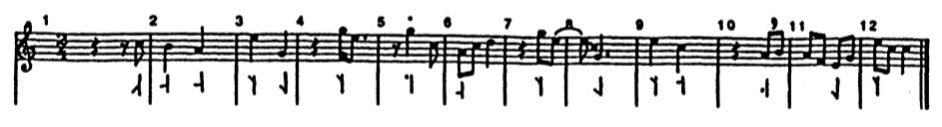
\includegraphics[width=0.8\linewidth]{figures/comparative/opera.jpg}
    \caption{Excerpt from the Cantonese tune ``Chatjiching''.}
    \label{fig:opera}
\end{figure}

The degree of this kind of fit varies. A review covering ten different studies of songs in as many different languages with phonemic pitch, found that compatibility of melodic and prosodic interval direction ranged from 67\% in the lowest scoring study (the African language Shona) to 98\% in the highest (Cantonese). \parencite[270]{schellenbergDoesLanguageDetermine2012} 

However, which will prove an important insight, variability within languages is also large, and was in several studies found to depend in a predictable fashion on genre, in the widest sense of that word. \parencite[271]{schellenbergDoesLanguageDetermine2012} \textcite{listSpeechMelodySong1961} found that in Thai, mnemonic songs such as a ditty intended to teach the alphabet scored the highest and modern popular music scored lower, while traditional songs scored somewhere in between. Interestingly, formal recitation of Siamese classical verse as taught in high-school and universities, while showing a scaffolding of compatibility, in execution is peppered with melisms and euphonious ``nonsense'' syllables like an embellished \textit{cantus firmus}, making it hard to calculate the score. \parencite[21-24]{listSpeechMelodySong1961}

Many of the world's literatures, including the just mentioned Siamese, make use of phonemic tone as one of the dimensions regulated by verse forms. If there were indeed Greek lyric songs with responding accentuation, and Greek poets consequently tended to place certain phonemic tones at certain places in their metrical schemes, they would stand in good company with numerous other literary traditions. Below is an example of phonemic tone responsion used as structural marker in Swedish modernist iambic pentameter. Besides giving the abstracted accentual pattern separately, where A and G stand for `acute' and `grave', the text has been marked with the same primary and secondary accents as in the minimal pairs in the earlier example.

\begin{quote}
    A A G G A
\end{quote}

\begin{verse}
    och d\'{o}ck skall r\'{ä}ttens r\'{i}k\textsecstress e sk\'{ö}rd\textsecstress as n\'u (final line, strophe 1) \\
    Där t\'{o}rn blev b\'{e}n och \'{o}lj\textsecstress ans r\'{u}stn\textsecstress ing br\'{a}nn (first line, strophe 2)\footnote{Analysis adapted from \textcite{kornhallVersOchTonaccent1995}. The verse lines are from Erik Lindegren's poem \textit{Scherzando} (1947).}
\end{verse}

By far the most famous example of regulated tone is the so-called tonal patterning in Middle Chinese \textit{lüshi} verse from the Tang dynasty, which came to provide the impetus for metres regulating tone in many neighbouring Asian literatures, like the Vietnamese and the Thai. An example is provided in \autoref{fig:spring-scene}.\footnote{Tonal patterning scheme adapted from \textcite{caiHowReadChinese2008}.} Note how the tones have been grouped into two classes, to get clearer contrasts. Such ``binarisation'' of the accents in metrical and melodical contexts can be seen in the classical literature of several languages with more than two accents, such as Chinese and Thai. Because of the structural highlighting of acute and circumflex, the Greek use of accent in verse is also mainly binary.

\begin{figure}[ht]
    \centering
    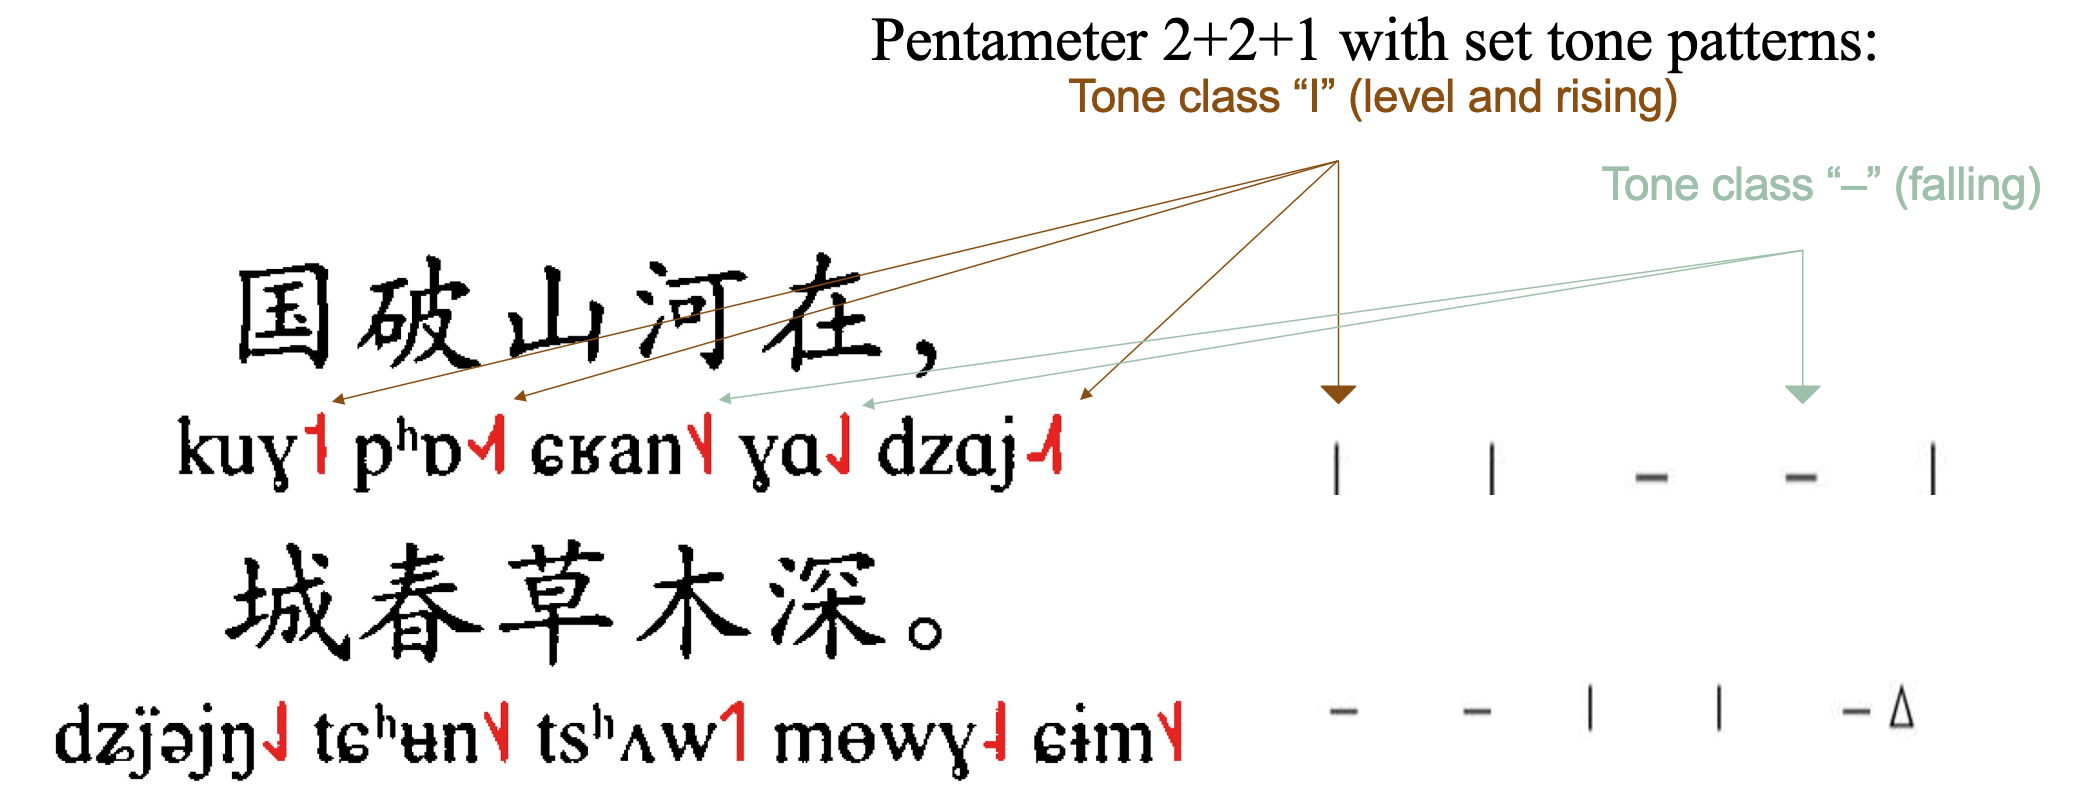
\includegraphics[width=1\linewidth]{figures/comparative/spring_scene.png}
    \caption{Excerpt from ``Spring scene" by Dù Fǔ (712–770).}
    \label{fig:spring-scene}
\end{figure}

%===============================================================
% Method

\section{Philological Theory}\label{sec:theory}

As promised in \autoref{sec:hist1} and \autoref{sec:hist2}, three metrics using the general methods of Wahlström, Abritta and Conser will now be defined, before being put to use in \autoref{sec:experiments}.

\subsection{Metric 1: Orthographic accent}\label{sec:orth}

The first metric is based on ``naive'' counting of accent signs, just like in \textcite{wahlstromAccentualResponsionGreek1970}.
In line with the standard treatment of it, the grave accent (`) turns out insignificant in all my tests, so the focus here will be on the metric for acutes (´) and circumflexes (\textasciicircum).
The metric is defined by the following ratio, where $n$ is the number of strophes: 

\[
M_1 \coloneqq \frac{n \times \text{(nr of sets of responding acutes/circumflexes)}}{\text{total nr of acutes/circumflexes in all strophes}}
\]

An example of counting responding orthographic accents is shown in \autoref{tab:clouds-orthographic} below.

\begin{table}[ht]
    \centering
    \resizebox{\textwidth}{!}{
        \begin{tabular}{c l l l}
            \hline
            V. & Strophe & Antistrophe & Metrical scheme \\
            \hline
            
            1 &
            \textgreek{ἀ\textcolor{red}{έ}ναοι Νε\textcolor{red}{φέ}λαι,} &
            \textgreek{παρ\textcolor{red}{θέ}νοι ὀμβρο\textcolor{red}{φό}ροι,} &
            $\longa\brevis(A)\brevis\longa\brevis\brevis(A)\longa$ \\
            
            2 &
            \makecell[l]{\textgreek{ἀρ\textcolor{red}{θῶ}μεν φανεραὶ \textbackslash}\\
                         \textgreek{δροσερὰν \textcolor{red}{φύ}σιν εὐ\textcolor{red}{ά}γητον}} &
            \makecell[l]{\textgreek{\textcolor{red}{ἔλ}θωμεν λιπαρὰν \textbackslash}\\
                         \textgreek{\textcolor{red}{χθό}να Παλ\textcolor{red}{λά}δο\textcolor{red}{ς, εὔ}ανδρον \textcolor{red}{γᾶν}}} &
            \makecell[l]{$\longa\longa\longa\brevis\brevis\longa$ \textbackslash\\
                         $\brevis\brevis\longa\brevis(A)\brevis\longa\longa\longa\longa$} \\
            
            3 &
            \textgreek{πατρὸς ἀπ᾽ Ὠκεα\textcolor{red}{νοῦ} βαρυαχ\textcolor{red}{έ}ος} &
            \textgreek{\textcolor{red}{Κέκ}ροπος ὑψ\textcolor{red}{ό}μεναι πολυ\textcolor{red}{ή}ρατον.} &
            $\longa\brevis\brevis\longa\brevis\brevis\longa\brevis\brevis\longa\brevis\brevis$ \\
            
            $\vdots$ & & & \\
            
            9 &
            \textgreek{μαρμα\textcolor{red}{ρέ}αισιν αὐ\textcolor{red}{γαῖς}.} &
            \textgreek{παντοδα\textcolor{red}{παῖ}σι\textcolor{red}{ν ὥ}ραις}, &
            $\longa\brevis\brevis\longa\brevis\longa\longa$ \\
            
            10 &
            \textgreek{ἀλλ᾽ ἀποσει\textcolor{red}{σά}μεναι \textcolor{red}{νέ}φο\textcolor{red}{ς ὄμ}βριον} &
            \textgreek{\textcolor{red}{ἦ}\textcolor{red}{ρί} τ᾽ ἐπερχο\textcolor{red}{μέ}νῳ Βρομ\textcolor{red}{ί}α \textcolor{red}{χά}ρις} &
            $\longa\brevis\brevis\longa\brevis\brevis\longa\brevis\brevis\longa\brevis\brevis$ \\
            
            11 &
            \textgreek{ἀθα\textcolor{red}{νά}τας ἰ\textcolor{red}{δέ}ας ἐπι\textcolor{red}{δώ}μεθα} &
            \textgreek{εὐκε\textcolor{red}{λά}δων τε χο\textcolor{red}{ρῶ}ν ἐρε\textcolor{red}{θίσ}ματα} &
            $\longa\brevis\brevis(A)\longa\brevis\brevis\longa\brevis\brevis\longa(A)\brevis\brevis$ \\
            
            12 &
            \textgreek{τηλεσ\textcolor{red}{κό}πῳ \textcolor{red}{ὄμ}ματι \textcolor{red}{γαῖ}αν.} &
            \textgreek{καὶ \textcolor{red}{μοῦ}σα βα\textcolor{red}{ρύβ}ρομος αὐ\textcolor{red}{λῶν}.} &
            $\longa\longa\brevis\brevis\longa(A)\brevis\brevis\longa\longa$ \\
            \hline
        \end{tabular}
    }
    \caption{Counting acute and circumflex accents in the \textit{parodos} of \textit{Nubes}. Syllables with accents are coloured red. Positions with responding accents are followed by ($A$) in the metrical scheme.}
    \label{tab:clouds-orthographic}
\end{table}

In the seven example lines shown in \autoref{tab:clouds-orthographic}, there are a total of forty-one syllables coloured red because they have acute or circumflex accents. Six pairs of them are found in identical positions in both strophe and antistrophe and thus count as responding. The result of calculating the metric is:

\[
M_1 = \frac{2 \times 6}{41} \approx 0.29
\]

\subsection{Metric 2: Phonological accent}\label{sec:barys}

It is by now well-established and relatively uncontroversial that the Greek pitch accent was accompanied by stress.\footnote{See \textcite{allenAccentRhythmProsodic1973} and his pertinent summary on p.\ 333f. Thanks to Andreas Keränen for pointing out both the existence of a modern optimality-theory derivation \parencite{blumenfeldTonetoStressStresstoToneAncient2004}, and that the pitch-stress hypothesis goes back all the way to \textcite{hilbergPrincipSilbenwagungUnd1879}.}
Stress was inversely correlated with pitch height and falls on syllables where the tone contour (``contonation'') lands. This means the following two types of syllable are stressed:
\begin{enumerate}
    \item syllable with circumflex, e.g. \textgreek{οῦ} in \textgreek{λυποῦ}
    \item long syllable following a syllable with an acute, e.g. \textgreek{ω} in \textgreek{λύω}
\end{enumerate}

With David (2006) this stress accent will be referred to as \textit{barys} (\textgreek{βαρύς}), a word that meant both ``deep'' and ``loud''.\footnote{As an example, in the \textit{parodos} of \textit{Nubes}, both the booming sound of the sea waves and the shrill \textit{aulos} pipes are described as \textit{barys}.}

The definition of the metric is the following ratio, where $n$ is the number of strophes:

\[
M_2 \coloneqq \frac{n \times \text{(nr of sets of responding \textit{barys} accents)}}{\text{total nr of \textit{barys} accents in all strophes}}
\]

An example of counting responding phonological accents is shown in \autoref{tab:clouds-barys}.

\begin{table}[ht]
    \centering
    \resizebox{\textwidth}{!}{
        \begin{tabular}{c l l l}
            \hline
            V. & Strophe & Antistrophe & Metrical scheme \\
            \hline
            
            1 &
            \textgreek{ἀέναοι Νεφέλ\textcolor{red}{αι},} &
            \textgreek{παρθένοι ὀμβροφό\textcolor{red}{ροι},} &
            $\longa\brevis\brevis\longa\brevis\brevis\longa(\beta)$ \\
            
            2 &
            \makecell[l]{\textgreek{ἀρ\textcolor{red}{θῶ}μεν φανεραὶ \textbackslash}\\
                         \textgreek{δροσερὰν φύσιν εὐά\textcolor{red}{γη}τον}} &
            \makecell[l]{\textgreek{ἔλ\textcolor{red}{θω}μεν λιπαρὰν \textbackslash}\\
                         \textgreek{χθόνα Παλλάδος, εὔ\textcolor{red}{αν}δρον \textcolor{red}{γᾶν}}} &
            \makecell[l]{$\longa\longa(\beta)\longa\brevis\brevis\longa$ \textbackslash\\
                         $\brevis\brevis\longa\brevis\brevis\longa\longa\longa\longa$} \\
            
            3 &
            \textgreek{πατρὸς ἀπ᾽ Ὠκεα\textcolor{red}{νοῦ} βαρυαχέος} &
            \textgreek{Κέκροπος ὑψόμεναι πολυήρατον.} &
            $\longa\brevis\brevis\longa\brevis\brevis\longa\brevis\brevis\longa\brevis\brevis$ \\
            
            $\vdots$ & & & \\
            
            9 &
            \textgreek{μαρμαρέ\textcolor{red}{αι}σιν αὐ\textcolor{red}{γαῖς}.} &
            \textgreek{παντοδα\textcolor{red}{παῖ}σιν ὥ\textcolor{red}{ραις},} &
            $\longa\brevis\brevis\longa(\beta)\brevis\longa\longa(\beta)$ \\
            
            10 &
            \textgreek{ἀλλ᾽ ἀποσεισάμεναι νέφος ὄμβριον} &
            \textgreek{\textcolor{red}{ἦ}ρί τ᾽ ἐπερχομέ\textcolor{red}{νῳ} Βρομί\textcolor{red}{α} χάρις} &
            $\longa\brevis\brevis\longa\brevis\brevis\longa\brevis\brevis\longa\brevis\brevis$ \\
            
            11 &
            \textgreek{ἀθανά\textcolor{red}{τα}ς ἰδέ\textcolor{red}{α}ς ἐπιδώμεθα} &
            \textgreek{εὐκελά\textcolor{red}{δων} τε χο\textcolor{red}{ρῶ}ν ἐρεθίσματα} &
            $\longa\brevis\brevis\longa(\beta)\brevis\brevis\longa(\beta)\brevis\brevis\longa\brevis\brevis$ \\
            
            12 &
            \textgreek{τηλεσκόπῳ ὄμματι \textcolor{red}{γαῖ}αν.} &
            \textgreek{καὶ \textcolor{red}{μοῦ}σα βαρύβρομος αὐ\textcolor{red}{λῶν}.} &
            $\longa\longa\brevis\brevis\longa\brevis\brevis\longa\longa$ \\
            \hline
        \end{tabular}
    }
    \caption{Counting \textit{barys} accents in the \textit{parodos} of \textit{Nubes}. Syllables with \textit{barys} accents are coloured red. Positions with responding \textit{barys} accents are followed by ($\beta$) in the metrical scheme.}
    \label{tab:clouds-barys}
\end{table}

In the seven example lines shown in \autoref{tab:clouds-barys}, there are a total of twenty-two syllables coloured red because they have \textit{barys} accents. Six pairs of them are found in identical positions in both strophe and antistrophe and thus count as responding. Calculating the metric yields the quotient:

\[
M_2 = \frac{2 \times 6}{22} = \frac{6}{11} \approx 0.55
\]

\subsection{Metric 3: Melodic accent}\label{sec:mel}

Since at least \textcite{crusiusNeuentdektenAntikenMusikresten1883}, philologists have been using the extant Greek musical fragments to induce rules by which the pitch accents of the lyrics restrict the melodic contour.\footnote{`Contour' here means the directions (rising, falling or neither) of the intervals, with their specific sizes unrestricted.} Three of the most important of these rules have been chosen by Conser as a basis for her operationalisation of contour.\footnote{For more on compatibility rules, see \textcite{cosgroveMelodyWordAccent2006}.}

These three rules can all be exemplified in the snippet from the beginning of Seikilos' epitaph found in \autoref{fig:seikilos}, copied from \textcite{westAncientGreekMusic1994}. To begin with, the fundamental ``Pitch Height Rule'' says that within one and the same word, the melody never reaches a higher point than on the syllable bearing the primary accent.\footnote{Through sandhi effects, polysyllabic words can sometimes have two accents. In that case, the first one is the primary.} Note that it says \textit{higher}—the melody is allowed to reach the \textit{same} point more than once, as it does in the word ``\textit{és-ti}'', melismatically set to B4-C5-B4 (in West's transcription from ancient to modern musical notation).

The second and third rules regulate when the melody rises and falls: ``pre-accentual rise'' means that the melody tends to rise before all three accents, i.e.\ the interval between an accented syllable and the preceding one is rising. This rise is seen for acute in ``\textit{o-lí}'' set to B4-D5, for circumflex in ``\textit{to-zzê-}'' set to G4-A4 and for grave in ``\textit{medèn}'' set to B4-C5. ``Post-accentual fall'' means that the melody tends to fall after acute and circumflex, but not after grave; this fall is exemplified in the first line for acute in ``\textit{sý ly}'' set to A4-G4, melismatically for circumflex in ``\textit{poû}'' set to A4-F4 and for grave in ``\textit{dèn ho}'' set to the non-falling C5-D5.

\begin{figure}[htbp]
    \centering
    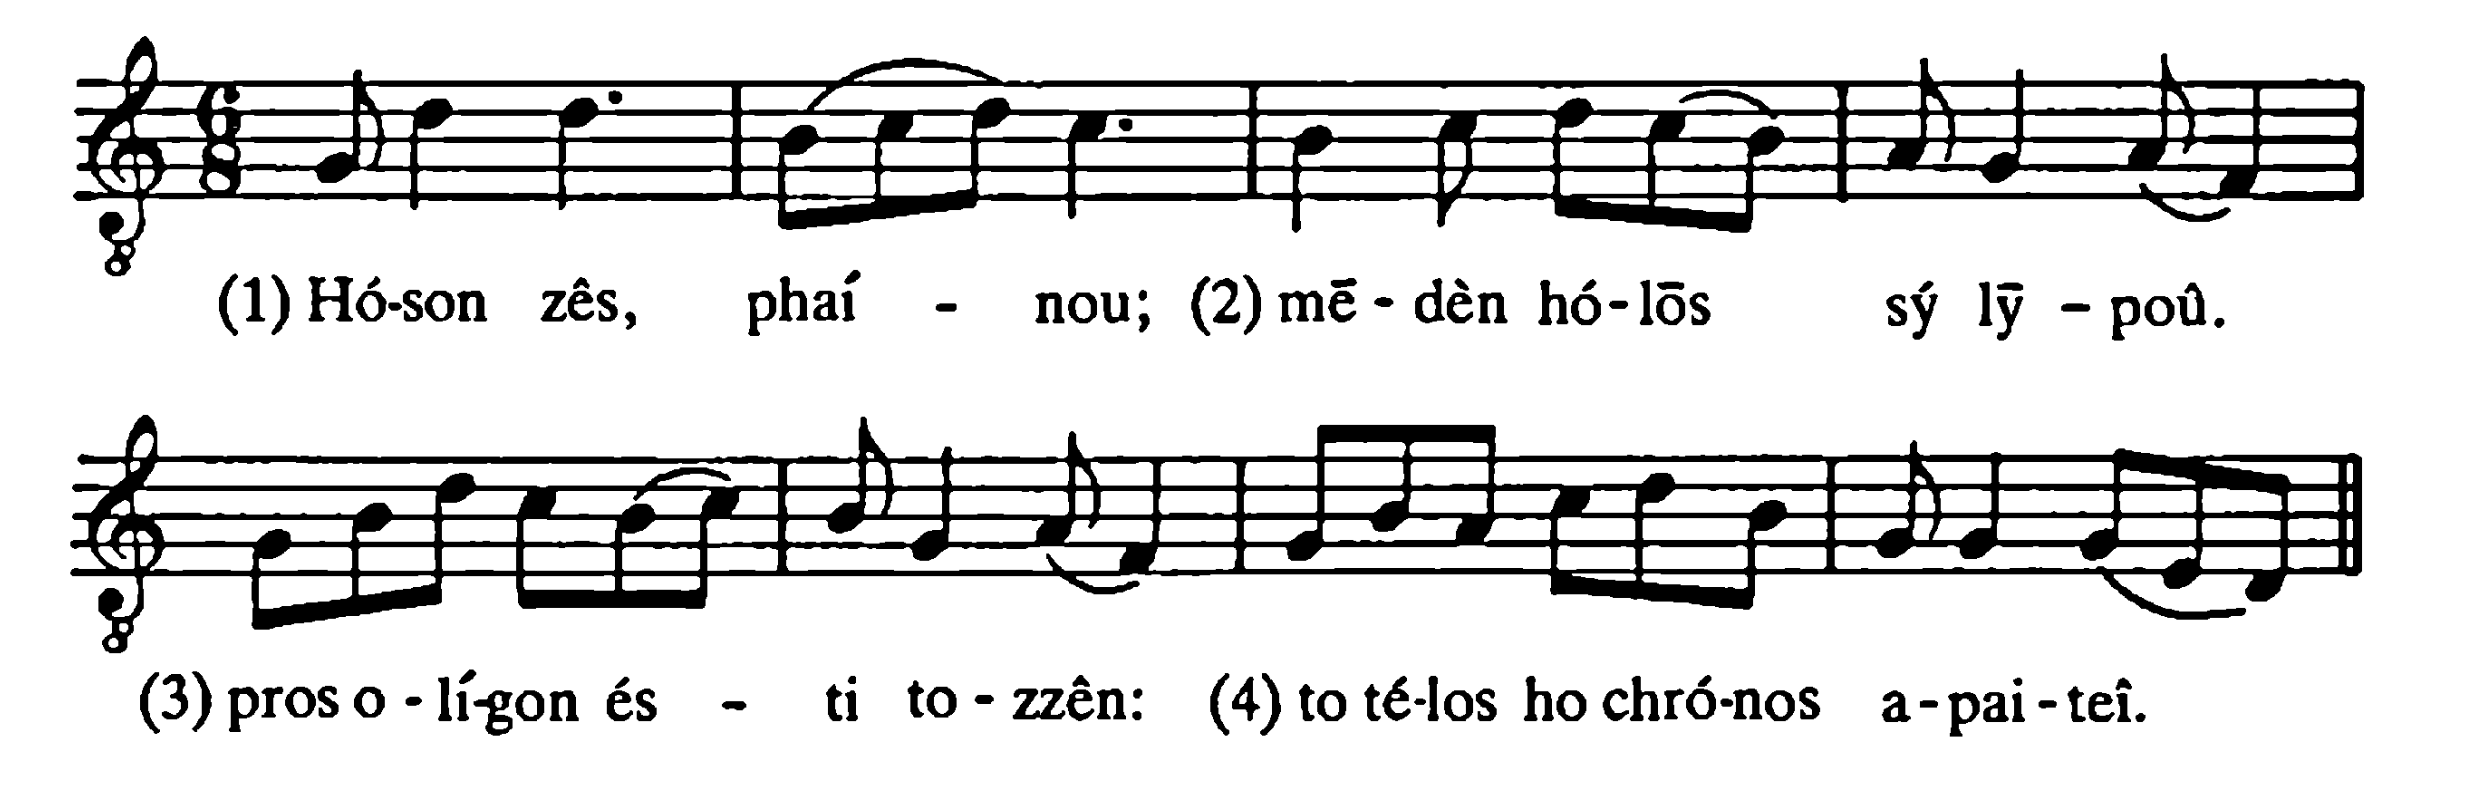
\includegraphics[width=1\linewidth]{figures/seikilos.png}
    \caption{Seikilos epitaph as transcribed in \textcite[301]{westAncientGreekMusic1994}, with my correction of an acute to a grave in ``medèn'', in line with \textcite[89]{westDocumentsAncientGreek2001}}
    \label{fig:seikilos}
\end{figure}

By these rules, any line of Greek can be deterministically mapped to a series of the following five contours or contour intervals:

\begin{enumerate}
  \item DN-A: Melody falls after primary acute or circumflex.
  \item DN: Melody falls after non-primary accent.
  \item UP: Melody rises before the acute or circumflex accent.
  \item UP-G: Melody rises before the grave.
  \item N: No restrictions on the contour (``flat'' or ``resting'').
\end{enumerate}

Melodic compatibility can then be defined as follows: two responding positions are melodically incompatible if one rises while the other falls. They are melodically compatible if they are not incompatible. In terms of the above five contours, the definition can be formalized as two positions being compatible if they both belong to either the ``up'' set \{DN-A, DN, N\} or the ``down'' set \{UP, UP-G, N\}.

The above mentioned rules concern how prosody restricts melody. Finally, the exception to the above rules must be mentioned: repeating pitches can be inserted at any point without being considered breaking the prosody, as a flat melodic interval is going neither up nor down. The musical fragments make use of such repetitions after 22\% of all notes. \parencite[265]{conserPitchAccentMelody2020}

Conser's original metric is binary and yields a 1 if all strophes are compatible and a 0 otherwise. In this paper, Conser’s metric is extended to rational scores in order to accommodate songs with more than two strophes in a more intuitive way. Given a set of two or more responding contours, the raw score for a position is calculated in the following way:

\begin{enumerate}
    \item Count the number of ``up'' contours, then count the number of ``down'' contours.
    
    \item Add the number of repeating N contours to the larger of the two counts, then divide that by the total number of responding contours.
\end{enumerate}

However, the minimum raw score will be larger in songs with more strophes. To enable direct score comparison both between songs with different strophicities and with Conser's binary scores, the final metric is normalised to be between 0 and 1. Since the normalisation is relative to song strophicity, the normalised score must be calculated in batches of one song at a time. The normalisation is done by subtracting the minimal score possible for the strophicity in question, and dividing the span, i.e.\ the difference between the maximal score (which is always 1) and the minimal score:

\begin{align*}
    M_{3} &\coloneqq \frac{M_{raw} - \text{minimal score}}{1 - \text{minimal score}}
\end{align*}

Let's take a three-strophic song and two raw scores of $\frac{2}{3}$ and $\frac{3}{3}$ as examples. In a three-strophic song $\frac{2}{3}$ is the minimum score, so the normalised scores will be respectively

\[
\frac{\frac{2}{3}-\frac{2}{3}}{\frac{1}{3}} = 0
\]
and
\[
\frac{\frac{3}{3}-\frac{2}{3}}{\frac{1}{3}} = 1,
\]
which was the desired outcome. Note that the $M_3$ compatibility metric of a line pair, a song, or a play is simply the mean of the $M_3$ metrics of all constituent positions.

An example of counting responding melodic contours is shown in \autoref{tab:clouds-contour}. Contours with strikethrough (e.g.\ \sout{UP}) indicate that there is incompatibility between the melodic direction of the strophe and the antistrophe.

\begin{table}[ht]
    \centering
    \resizebox{\textwidth}{!}{
        \begin{tabular}{c l l}
            \hline
            V. & Strophe & Antistrophe \\
            \hline
            
            1 &
            \makecell[l]{\textgreek{ἀέναοι Νεφέλαι,}\\
            UP, DN-A, DN, N, UP, DN-A, N} & % 7
            \makecell[l]{\textgreek{παρθένοι ὀμβροφόροι,}\\
            UP, DN-A, N, UP, UP, DN-A, N} \\

            \hline
            
            2 &
            \makecell[l]{\textgreek{ἀρθῶμεν φανεραὶ \textbackslash}\\
                         \textgreek{δροσερὰν φύσιν εὐάγητον}\\
            \sout{UP}, DN-A, N, UP, UP, UP-G,\\ 
            \sout{UP}, UP, UP-G, DN-A, N, \sout{UP}, DN-A, DN, N} & % 15
            \makecell[l]{\textgreek{ἔλθωμεν λιπαρὰν \textbackslash}\\
                         \textgreek{χθόνα Παλλάδος, εὔανδρον γᾶν}\\
            \sout{DN-A}, DN, N, UP, UP, UP-G,\\ 
            \sout{DN-A}, N, UP, DN-A, N, \sout{DN-A}, DN, N, N} \\

            \hline
            
            3 &
            \makecell[l]{\textgreek{πατρὸς ἀπ᾽ Ὠκεανοῦ βαρυαχέος}\\
            \sout{UP}, \sout{UP-G}, N, UP, \sout{UP}, \sout{UP}, N,\\ 
            UP, UP, \sout{UP}, DN-A, N} & % 12
            \makecell[l]{\textgreek{Κέκροπος ὑψόμεναι πολυήρατον.}\\
            \sout{DN-A}, \sout{DN}, N, UP, \sout{DN-A}, \sout{DN}, N,\\ 
            UP, UP, \sout{DN-A}, DN, N} \\
            
            $\vdots$ & & \\
            
            9 &
            \makecell[l]{\textgreek{μαρμαρέαισιν αὐγαῖς.}\\
            UP, UP, \sout{DN-A}, DN, N, \sout{UP}, N} & % 7
            \makecell[l]{\textgreek{παντοδαπαῖσιν ὥραις},\\
            UP, UP, \sout{UP}, DN-A, N, \sout{DN-A}, N} \\

            \hline
            
            10 &
            \makecell[l]{\textgreek{ἀλλ᾽ ἀποσεισάμεναι νέφος ὄμβριον}\\
            N, UP, UP, UP, \sout{DN-A}, DN, N, \sout{DN-A}, N,\\ 
            DN-A, DN, N} & % 12
            \makecell[l]{\textgreek{ἦρί τ᾽ ἐπερχομένῳ Βρομία χάρις}\\
            DN-A, N, UP, UP, \sout{UP}, DN-A, N, \sout{UP}, DN-A,\\ 
            N, DN-A, N} \\

            \hline
            
            11 &
            \makecell[l]{\textgreek{ἀθανάτας ἰδέας ἐπιδώμεθα}\\
            UP, UP, DN-A, N, UP, \sout{DN-A}, N, UP, UP,\\
            DN-A, DN, N} & % 12
            \makecell[l]{\textgreek{εὐκελάδων τε χορῶν ἐρεθίσματα}\\
            UP, UP, DN-A, DN, N, \sout{UP}, N, UP, UP,\\ 
            DN-A, DN, N} \\

            \hline
            
            12 &
            \makecell[l]{\textgreek{τηλεσκόπῳ ὄμματι γαῖαν.}\\
            UP, \sout{UP}, DN-A, N, DN-A, DN, N, \sout{DN-A}, N} & % 9
            \makecell[l]{\textgreek{καὶ μοῦσα βαρύβρομος αὐλῶν.}\\
            UP-G, \sout{DN-A}, N, UP, DN-A, DN, N, \sout{UP}, N} \\
            \hline
        \end{tabular}
    }
    \caption{Checking melodic compatibility in the \textit{parodos} of \textit{Nubes}. Incompatible contours are struck out.}
    \label{tab:clouds-contour}
\end{table}

The information contained in the above contours is summarised in the metrical scheme in \autoref{tab:clouds-contour-scheme}, where red positions indicate compatibility and black contradiction.

\begin{table}[ht]
    \centering
    \begin{tabular}{c l}
        \hline
        V. & Metrical scheme \\
        \hline
        1 & $\textcolor{red}{\longa}\textcolor{red}{\brevis}\textcolor{red}{\brevis}\textcolor{red}{\longa}\textcolor{red}{\brevis}\textcolor{red}{\brevis}\textcolor{red}{\longa}$ \\
        
        2 & \makecell[l]{$\longa\textcolor{red}{\longa}\textcolor{red}{\longa}\textcolor{red}{\brevis}\textcolor{red}{\brevis}\textcolor{red}{\longa}$ \textbackslash\\
                           $\brevis\textcolor{red}{\brevis}\textcolor{red}{\longa}\textcolor{red}{\brevis}\textcolor{red}{\brevis}\longa\textcolor{red}{\longa}\textcolor{red}{\longa}\textcolor{red}{\longa}$} \\
        
        3 & $\longa\brevis\textcolor{red}{\brevis}\textcolor{red}{\longa}\brevis\brevis\textcolor{red}{\longa}\textcolor{red}{\brevis}\textcolor{red}{\brevis}\longa\textcolor{red}{\brevis}\textcolor{red}{\brevis}$ \\

        $\vdots$ & \\
        
        9 & $\textcolor{red}{\longa}\textcolor{red}{\brevis}\brevis\textcolor{red}{\longa}\textcolor{red}{\brevis}\longa\textcolor{red}{\longa}$ \\
        
        10 & $\textcolor{red}{\longa}\textcolor{red}{\brevis}\textcolor{red}{\brevis}\textcolor{red}{\longa}\brevis\textcolor{red}{\brevis}\textcolor{red}{\longa}\brevis\textcolor{red}{\brevis}\textcolor{red}{\longa}\textcolor{red}{\brevis}\textcolor{red}{\brevis}$ \\
        
        11 & $\textcolor{red}{\longa}\textcolor{red}{\brevis}\textcolor{red}{\brevis}\textcolor{red}{\longa}\textcolor{red}{\brevis}\brevis\textcolor{red}{\longa}\textcolor{red}{\brevis}\textcolor{red}{\brevis}\textcolor{red}{\longa}\textcolor{red}{\brevis}\textcolor{red}{\brevis}$ \\
        
        12 & $\textcolor{red}{\longa}\longa\textcolor{red}{\brevis}\textcolor{red}{\brevis}\textcolor{red}{\longa}\textcolor{red}{\brevis}\textcolor{red}{\brevis}\longa\textcolor{red}{\longa}$ \\
        \hline
    \end{tabular}
    \caption{Melodic compatibility (red) or contradiction (black) per metrical position}
    \label{tab:clouds-contour-scheme}
\end{table}

Intuitively, the metric can be calculated by dividing the number of red positions in the above metrical scheme by the total number of positions. Using the formal definition:

\[
M_3 = \frac{2 \times 26}{74} = \frac{59}{74} \approx 0.80
\]

The intended interpretation is that 80\% of the time, the direction of the melodic contours of the example lines from the strophe do not contradict those of the antistrophe. 

%===============================================================
% Results

\section{Statistical Experiments}\label{sec:experiments}

The corpus of Aristophanes' strophic songs (i.e.\ songs with refrains) consists of seventy-eight songs. \autoref{tab:comedies} shows the distribution of songs over the eleven extant plays.\footnote{Conventional Latin names and abbreviations of ancient plays in this paper are those used in the LSJ. \textit{Equites} is notable in that out of the eleven it is the only play whose songs are all strophic.}

\begin{table}[htbp]
    \centering
    \begin{tabular}{l l l}
        \hline
        Play                               & Strophic Songs & Polystrophic Songs          \\
        \hline
        \textit{Acharnienses}              & 9              & 1 (four strophes)           \\
        \textit{Equites}                   & 8              & 1 (four strophes)           \\
        \textit{Nubes}                     & 6              & --                          \\
        \textit{Vespae}                    & 8              & --                          \\
        \textit{Pax}                       & 6              & 1 (three strophes)          \\
        \textit{Aves}                      & 10             & --                          \\
        \textit{Lysistrata}                & 8              & 1 (four strophes)           \\
        \textit{Thesmophoriazusae}         & 4              & --                          \\
        \textit{Ranae}                     & 11             & 2 (three and four strophes) \\
        \textit{Ecclesiazusae}             & 6              & --                          \\
        \textit{Plutus}                    & 2              & --                          \\
        \hline
        Total                              & 78             & 6                           \\
        \hline
    \end{tabular}
    \caption{Aristophanes' strophic songs}
    \label{tab:comedies}
\end{table}

The seventy-eight songs together comprise 6 604 sets of responding metrical positions, and has been manually supplied with XML markup indicating syllable boundaries, syllable weight, pairs of resolved light syllables, anceps as well as names for the metre of each line. Lines with textual problems affecting the prosody and metrical responsion have been excluded, following the philological judgement of \textcite{parkerSongsAristophanes1997}, \textcite{wilsonAristophanisFabulaeTomus2007} and \textcite{wilsonAristophanisFabulaeTomus2007a}. It is the first time a large open-source database of scanned Aristophanes is made available. 

From the point of view of statistical theory, these 6 604 sets are our random variables. 

\subsection{Baselines}

Two genres of baseline will be used, and three strophicities for each genre (two-strophic, three-strophic and four-strophic). The first genre consists of fifty-two lines of Aristophanes' dialogue iambic trimeters and the second of all forty-six lines of lyric trochaic tetrameters present in the corpus.\footnote{The iambic trimeters are selected at random from the beginning of \textit{Acharnians}, excluding lines that feature ``comic anapaests'' which break responsion.} Since the tetrameters come from responding songs, care is necessary when combining them. It is important that no lines that respond in a baseline are actually \textit{in situ} responding lines.

The baseline corpus used for the permutation tests mirrors the shape of the corpus of Aristophanes: it contains seventy-eight baseline songs, seventy-two of which are permutations of the two-strophic, two of which are permutations of the three-strophic and four of which are permutations of the four-strophic. This whole set of seventy-eight songs is having its lines permuted one thousand times while making sure firstly that no permutations are identical and secondly that the same stricture holds for each permutation that held for the first constructed baselines, namely that no originally responding lines respond.

\subsection{Chronological correlations}\label{sec:chrono}

\textcite{conserPitchAccentMelody2020} shows that given the standard dating, the plays of Aeschylus show a clear tendency for linear growth of melodic compatibility over time, meaning that in general his plays have higher scores later in his career.\footnote{The four plays by Sophocles whose scores are calculated in \textcite{conserAiolaNuxMusical2024} are not useful for linear regression, since their chronological ordering is too contested. Cf.\ Conser's footnote 17.} This hypothesis is intuitively captured in \autoref{fig:linreg-aeschylus}, which shows a linear regression calculated on the numbers in Conser's article, yielding a ``huge'' effect size.\footnote{In this paper, all linear regressions and their r-values are calculated with the \texttt{scipy.stats} Python package, and all the interpretations of the effect sizes follow the modern standard of \textcite{sawilowskyNewEffectSize2009}.}

\begin{figure}
    \centering
    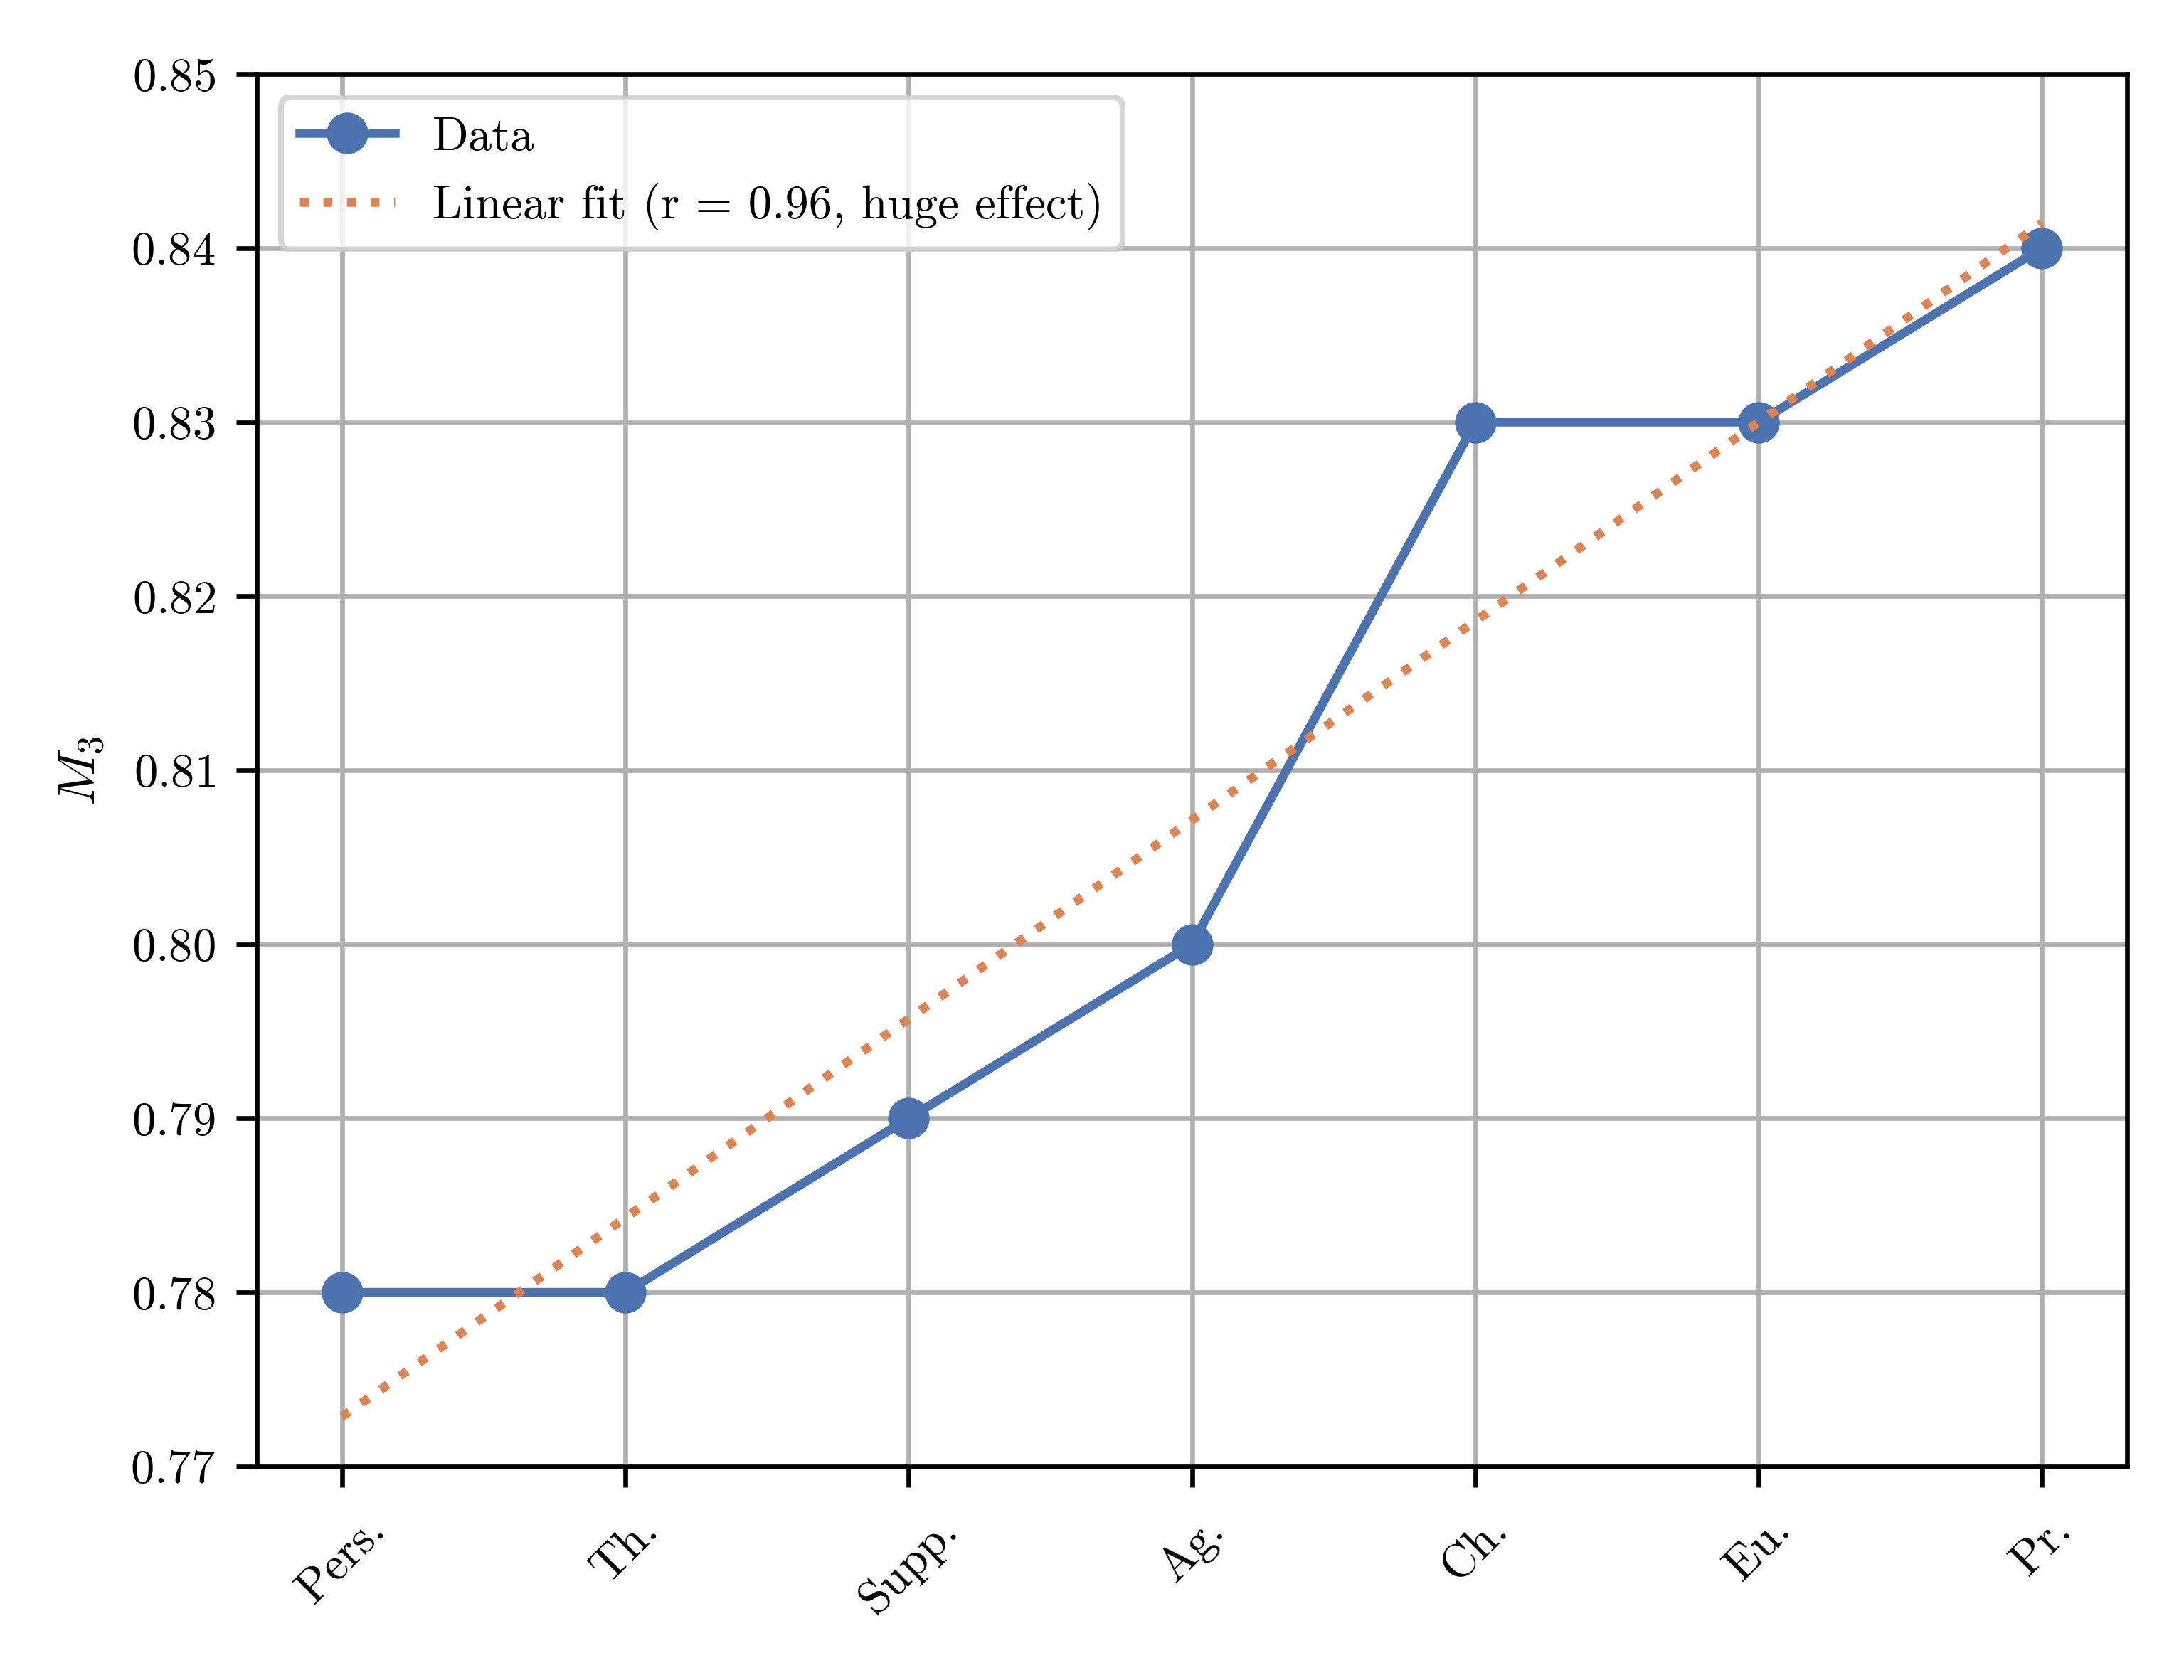
\includegraphics[width=1\linewidth]{figures/play_regression/linreg_aeschylus.png}
    \caption{Melodic compatibility over time in Aeschylus' tragedies \parencite{conserPitchAccentMelody2020}}
    \label{fig:linreg-aeschylus}
\end{figure}

\autoref{fig:linreg-comp} shows the \textit{prima facie} confusing results of performing the same calculations for Aristophanes. The positive linearity hinges on the leverage of the large outlier score of the final play \textit{Plutus} (acronym ``Pl.'' in the figures), as the influence a data point has on the slope of a linear regression line correlates directly not only with the size of its $y$, but also with the distance of the point from the $x$ mean.
\begin{figure}
    \centering
    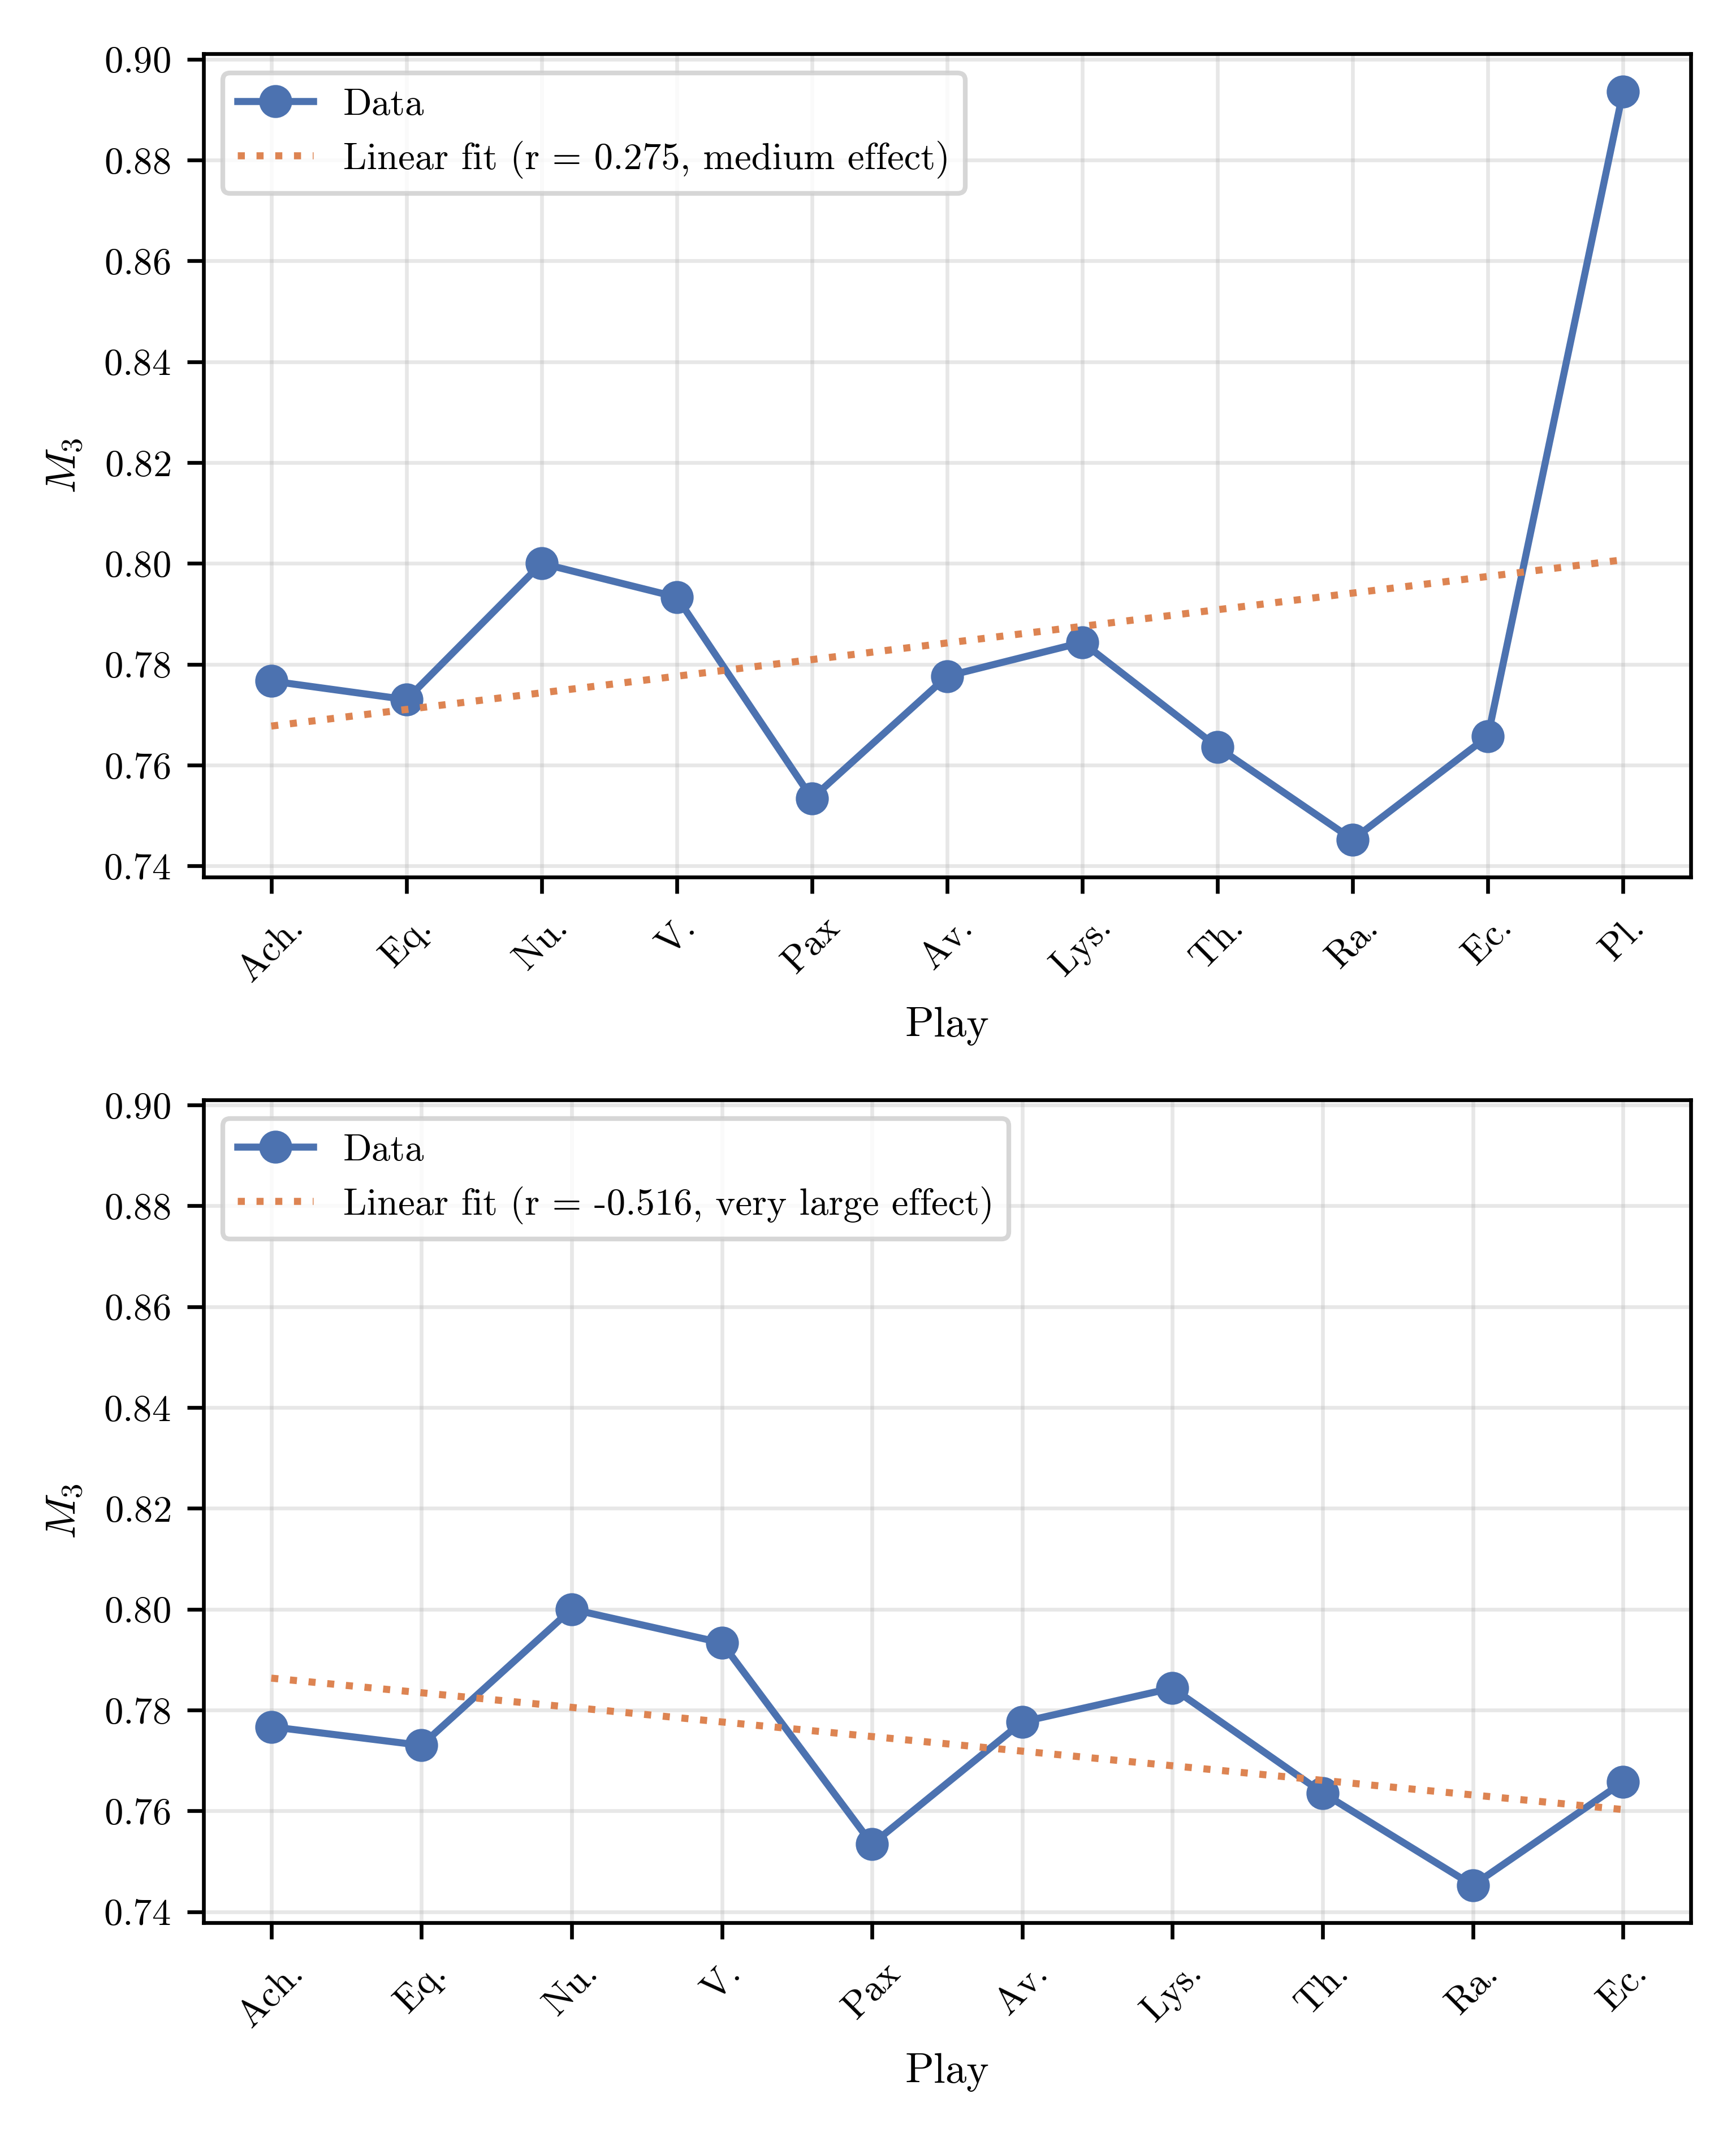
\includegraphics[width=1\linewidth]{figures/play_regression/linreg_comp.png}
    \caption{Melodic compatibility over time in Aristophanes' comedies. In the lower plot his last play \textit{Plutus} (with the acronym ``Pl.'') is excluded.}
    \label{fig:linreg-comp}
\end{figure}

When considered without \textit{Plutus}, the linear model for the melodic metric of the comedies not only sheds its positive slope but instead shows a \textit{negative} inclination with a stronger effect size than the positive had been, although it is still just half that of the ``huge'' effect size of Aeschylus' linear model. The same general phenomenon, namely a shift from positive to negative slope, can be seen in the plot pairs for the other two metrics in \autoref{fig:linreg-barys} and \autoref{fig:linreg-comp}, although with noticeably less effect size (``small'' and ``large'' respectively). 

Clearly, it is necessary to perform an outlier analysis on \textit{Plutus}, asking what factors contribute to its large score, before it can plausibly be removed from the regression.

\begin{figure}
    \centering
    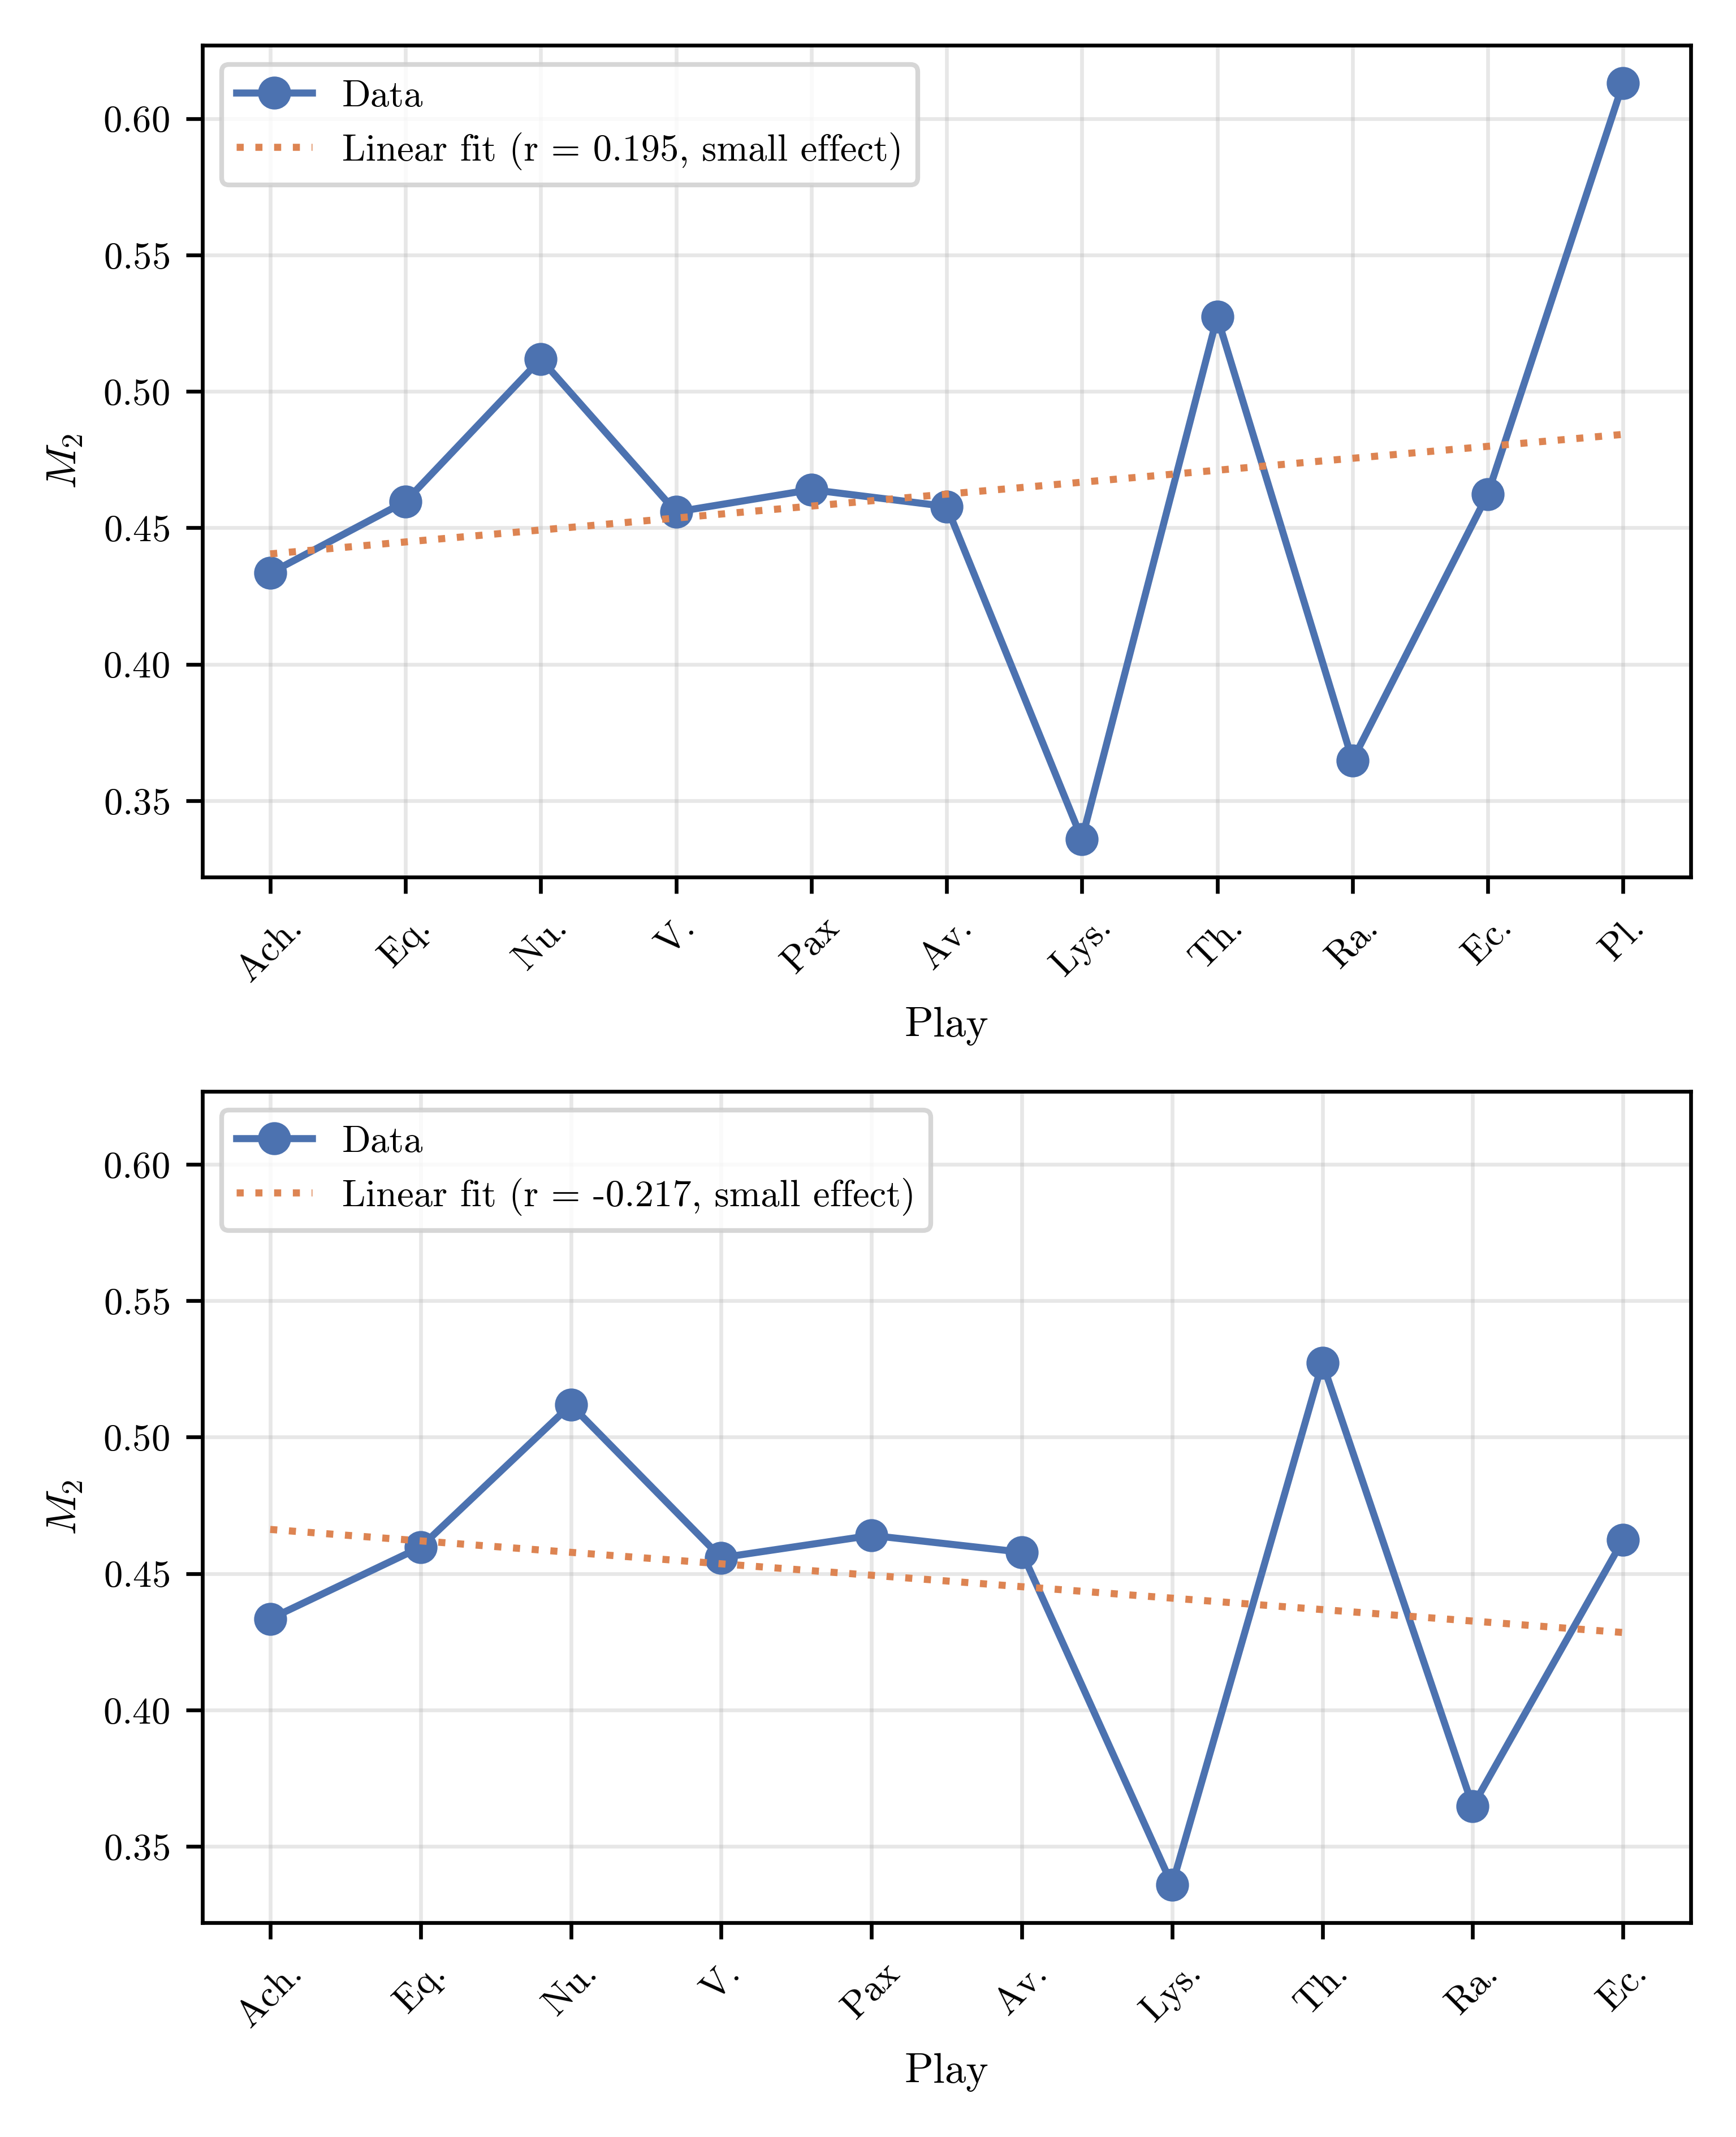
\includegraphics[width=1\linewidth]{figures/play_regression/linreg_barys.png}
    \caption{\textit{Barys} responsion ($M_2$) over time in Aristophanes' comedies. In the lower plot his last play \textit{Plutus} (with the acronym ``Pl.'') is excluded.}
    \label{fig:linreg-barys}
\end{figure}
\begin{figure}
    \centering
    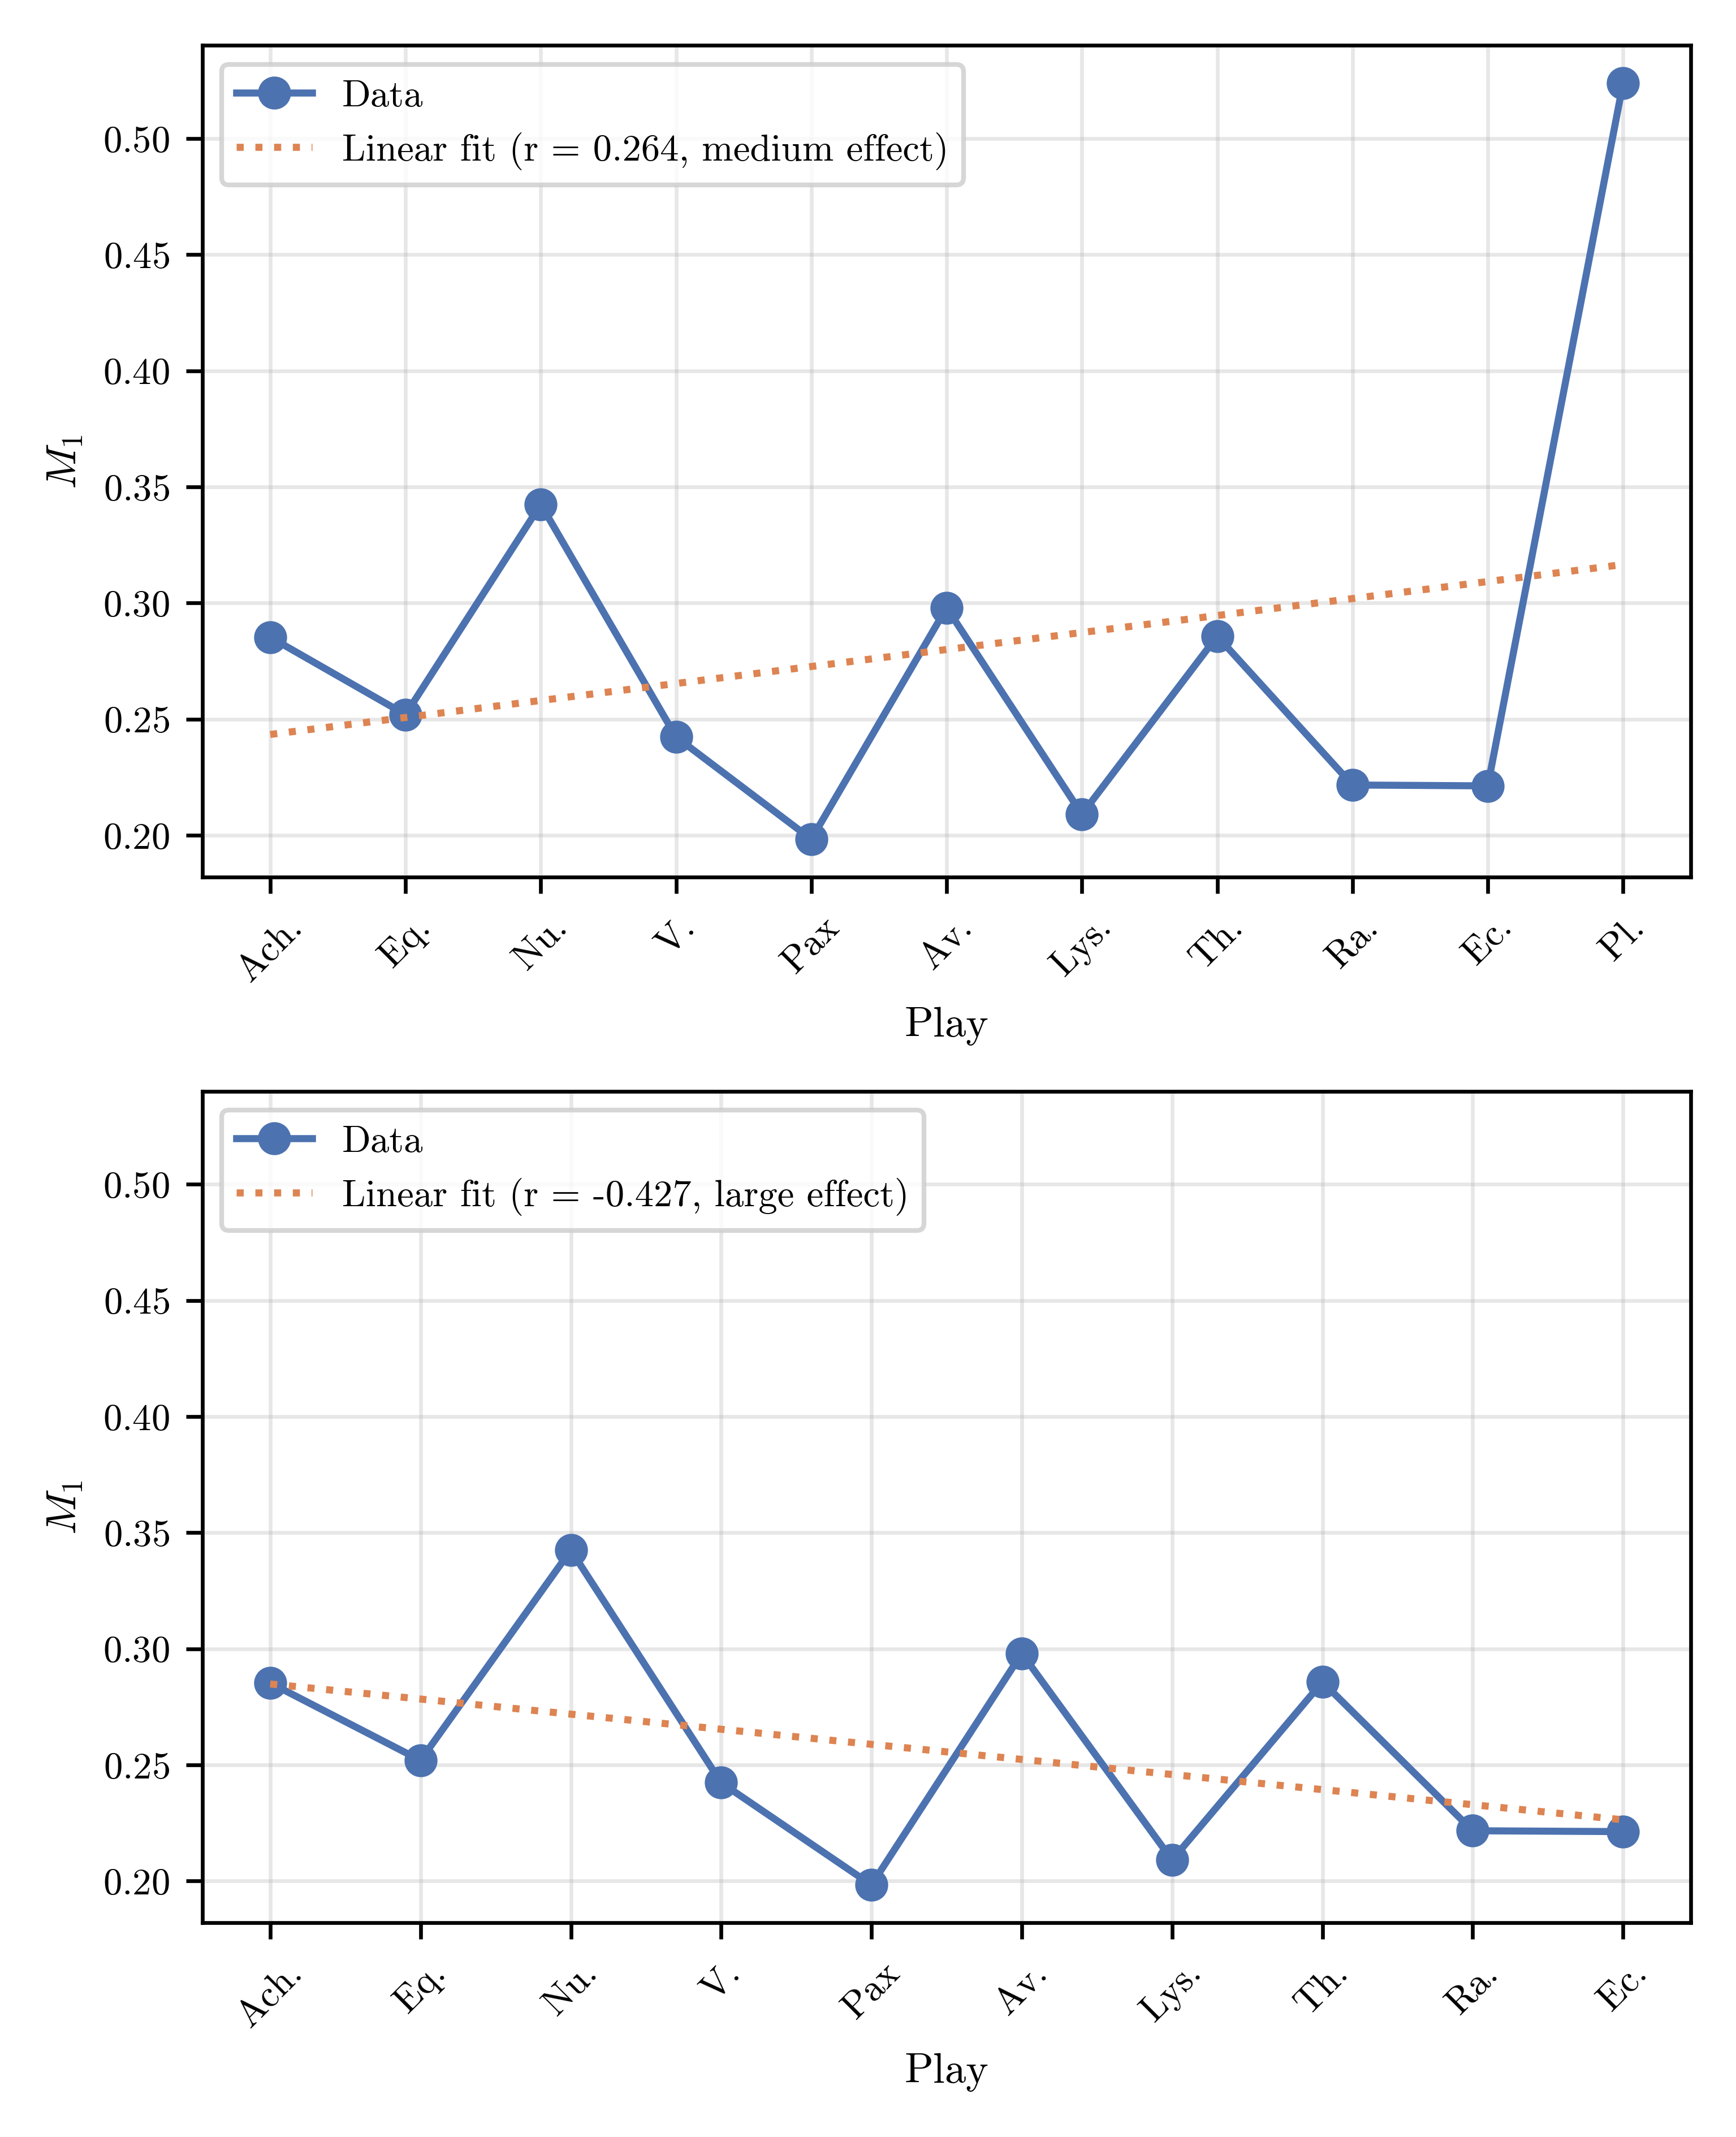
\includegraphics[width=1\linewidth]{figures/play_regression/linreg_orth.png}
    \caption{Orthographic responsion ($M_1$ over time in Aristophanes' comedies. In the lower plot his last play \textit{Plutus} (with the acronym ``Pl.'') is excluded.}
    \label{fig:linreg-orth}
\end{figure}

The most obvious factor is that \textit{Plutus} is Aristophanes’ last play, which gives it leverage on the $x$-axis. But it is also the play with the fewest songs, and having few songs means statistical instability and increased score vulnerability to outlier songs, which leads to leverage on the $y$-axis as well. 

The question thus reduces to whether there is anything special about \textit{Plutus} and its two responding lyric songs. The answer is yes: \textit{Plutus} is well known to have broken with the earlier role of the chorus as constant commentator, and the play's use of lyric is restricted to a single ``set-piece'' of two songs. \parencite[555]{parkerSongsAristophanes1997}. 

This set-piece has four characteristics that can be used to explain the exceptional melodic-prosodic compatibility, and which are all orthogonal to the underlying stylistic development that the linear test is attempting to look for. The characteristics are given in order from less to more significant. 

First, the two songs of \textit{Plutus} are both antistrophic, and as we’ve seen, polystrophy means responding less in all ways. Second, they constitute the four verses of a ``diegetic'' (story-world) song: the characters explicitly say that they are lampooning a known song, identified by scholiasts as Philoxenus’ ``Cyclops and Galatea''. Third, the protagonist Karion singing the strophe explicitly urges the chorus to ``follow'' him in the antistrophe, and both strophes strongly affirm that they sing to the melody of the ``Cyclops''. Hence this is an extremely rare case where it can be very confidently asserted that the strophes were sung to the same melody. Fourth, in each of the songs, the last half of the first line of both refrains is identical, surely a quotation of the original song. Exact repetition warps the statistics by yielding perfect scores, since the resulting automatic prosodic alignment is completely irrelevant to the investigated phenomenon, which is the actively careful accent distribution of otherwise differing words and phrases.

\subsection{Corpus scores}

The results of computing all three metrics on the full corpus are given in \autoref{tab:general-results}, with the melodic compatibility of Aeschylus from \textcite{conserPitchAccentMelody2020} included as comparison.

\begin{table}[ht]
    \centering
    \begin{tabular}{l c}
        \hline
                                             & Observed value \\
        \hline
         $M_1$ (Acute-circumflex responsion) & 0.26 \\
         $M_2$ (\textit{Barys} responsion)   & 0.44 \\
         $M_3$ (Melodic compatibility)       & 0.82 \\
         \hline
    \end{tabular}
    \caption{Full-corpus metrics}
    \label{tab:general-results}
\end{table}

The outlier analysis in \autoref{sec:chrono} showed that the metric scores are boosted by \textit{Plutus} in a way that threatens to render the results unconvincing. Hence, all metrics have been calculated again for a corpus with \textit{Plutus} removed. \autoref{tab:general-results-no-pl} gives the results of the orthographic and \textit{barys} metrics, with the acute-circumflex orthographic result for Aeschylus' seven tragedies from \textcite[265]{conserPitchAccentMelody2020} as comparison, and \autoref{tab:m3-results-no-pl} gives the melodic metric and compares it with the results for Aeschylus (\textit{loc}.\ \textit{cit}.) as well as four tragedies by Sophocles from \textcite[110]{conserAiolaNuxMusical2024}. The highest and lowest scoring languages in the ethnomusicological study \textcite[270]{schellenbergDoesLanguageDetermine2012} mentioned in \autoref{sec:comparative} are appended at the end to make clear that all the Greek poets' scores are plausible in the sense that they fall within the span of other tonal languages.\footnote{Just like the metric adapted from Conser used in this paper, the studies in Schellenberg report non-contradiction of interval direction calculated per syllable, so the numbers are directly comparable.}

\begin{table}[ht]
    \centering
    \begin{tabular}{l c}
        \hline
                                            & Observed value \\
        \hline
        $M_1$ (Acute-circumflex responsion) & 0.25 \\
        $M_2$ (\textit{Barys} responsion)   & 0.43 \\
        \hline
                                            & Comparative value \\
        \hline
        $M_1$ Aeschylus                     & 0.13 \\
        \hline
    \end{tabular}
    \caption{Orthographic and \textit{barys} metrics on the corpus without \textit{Pl}.}
    \label{tab:general-results-no-pl}
\end{table}

\begin{table}[ht]
    \centering
    \begin{tabular}{l c}
        \hline
                                           & Observed value \\
        \hline
        Aristophanes (except \textit{Pl}.)& 0.77 \\
        \hline
                                           & Comparative value \\
        \hline
        Aeschylus                         & 0.80 \\
        \textit{Ajax} (Soph.)               & 0.81 \\
        \textit{Antigone} (Soph.)          & 0.82 \\
        \textit{Trachiniae} (Soph.)         & 0.83 \\
        \textit{Oedipus Tyrannus} (Soph.)    & 0.83 \\
        Cantonese                         & 0.98 \\
        Shona                             & 0.67 \\
        \hline
    \end{tabular}
    \caption{Comparison of the melodic metrics of Aristophanes, Aeschylus, Sophocles and reference languages}
    \label{tab:m3-results-no-pl}
\end{table}

$M_1$ and $M_2$ are similar enough that an absolute numerical comparison is meaningful.  Not only are both counting a type of discrete accent that is guaranteed to be well-defined exclusively for bigger sets of positions like songs, but for every \textit{barys} accent there is an acute or a circumflex (but not vice verse), so the \textit{barys} are a proper subset of the orthographic accents. It therefore serves as tentative corroboration of the pitch-stress theory of the Greek accent that that the absolute score of the \textit{barys} beats the orthographic with such a wide margin. However, a second and more nuanced litmus test is found in \autoref{tab:perm} in \autoref{sec:perm}.

$M_3$, on the other hand, is a completely different metric, and a fair comparison between it and the other two metrics will only become possible with the statistical tests of significance.

\subsection{Permutation tests}\label{sec:perm}

A comparison of the observed corpus metrics and the distribution of one thousand test statistics calculated on the permuted corpora are presented in \autoref{fig:orth-perm}, \autoref{fig:barys-perm} and \autoref{fig:comp-perm} for the orthographic, \textit{barys} and melodic compatibility metrics respectively. To make the test harder and the significance more robust, the three observed metrics used are the lower scores that exclude \textit{Plutus}.

\begin{figure}
    \centering
    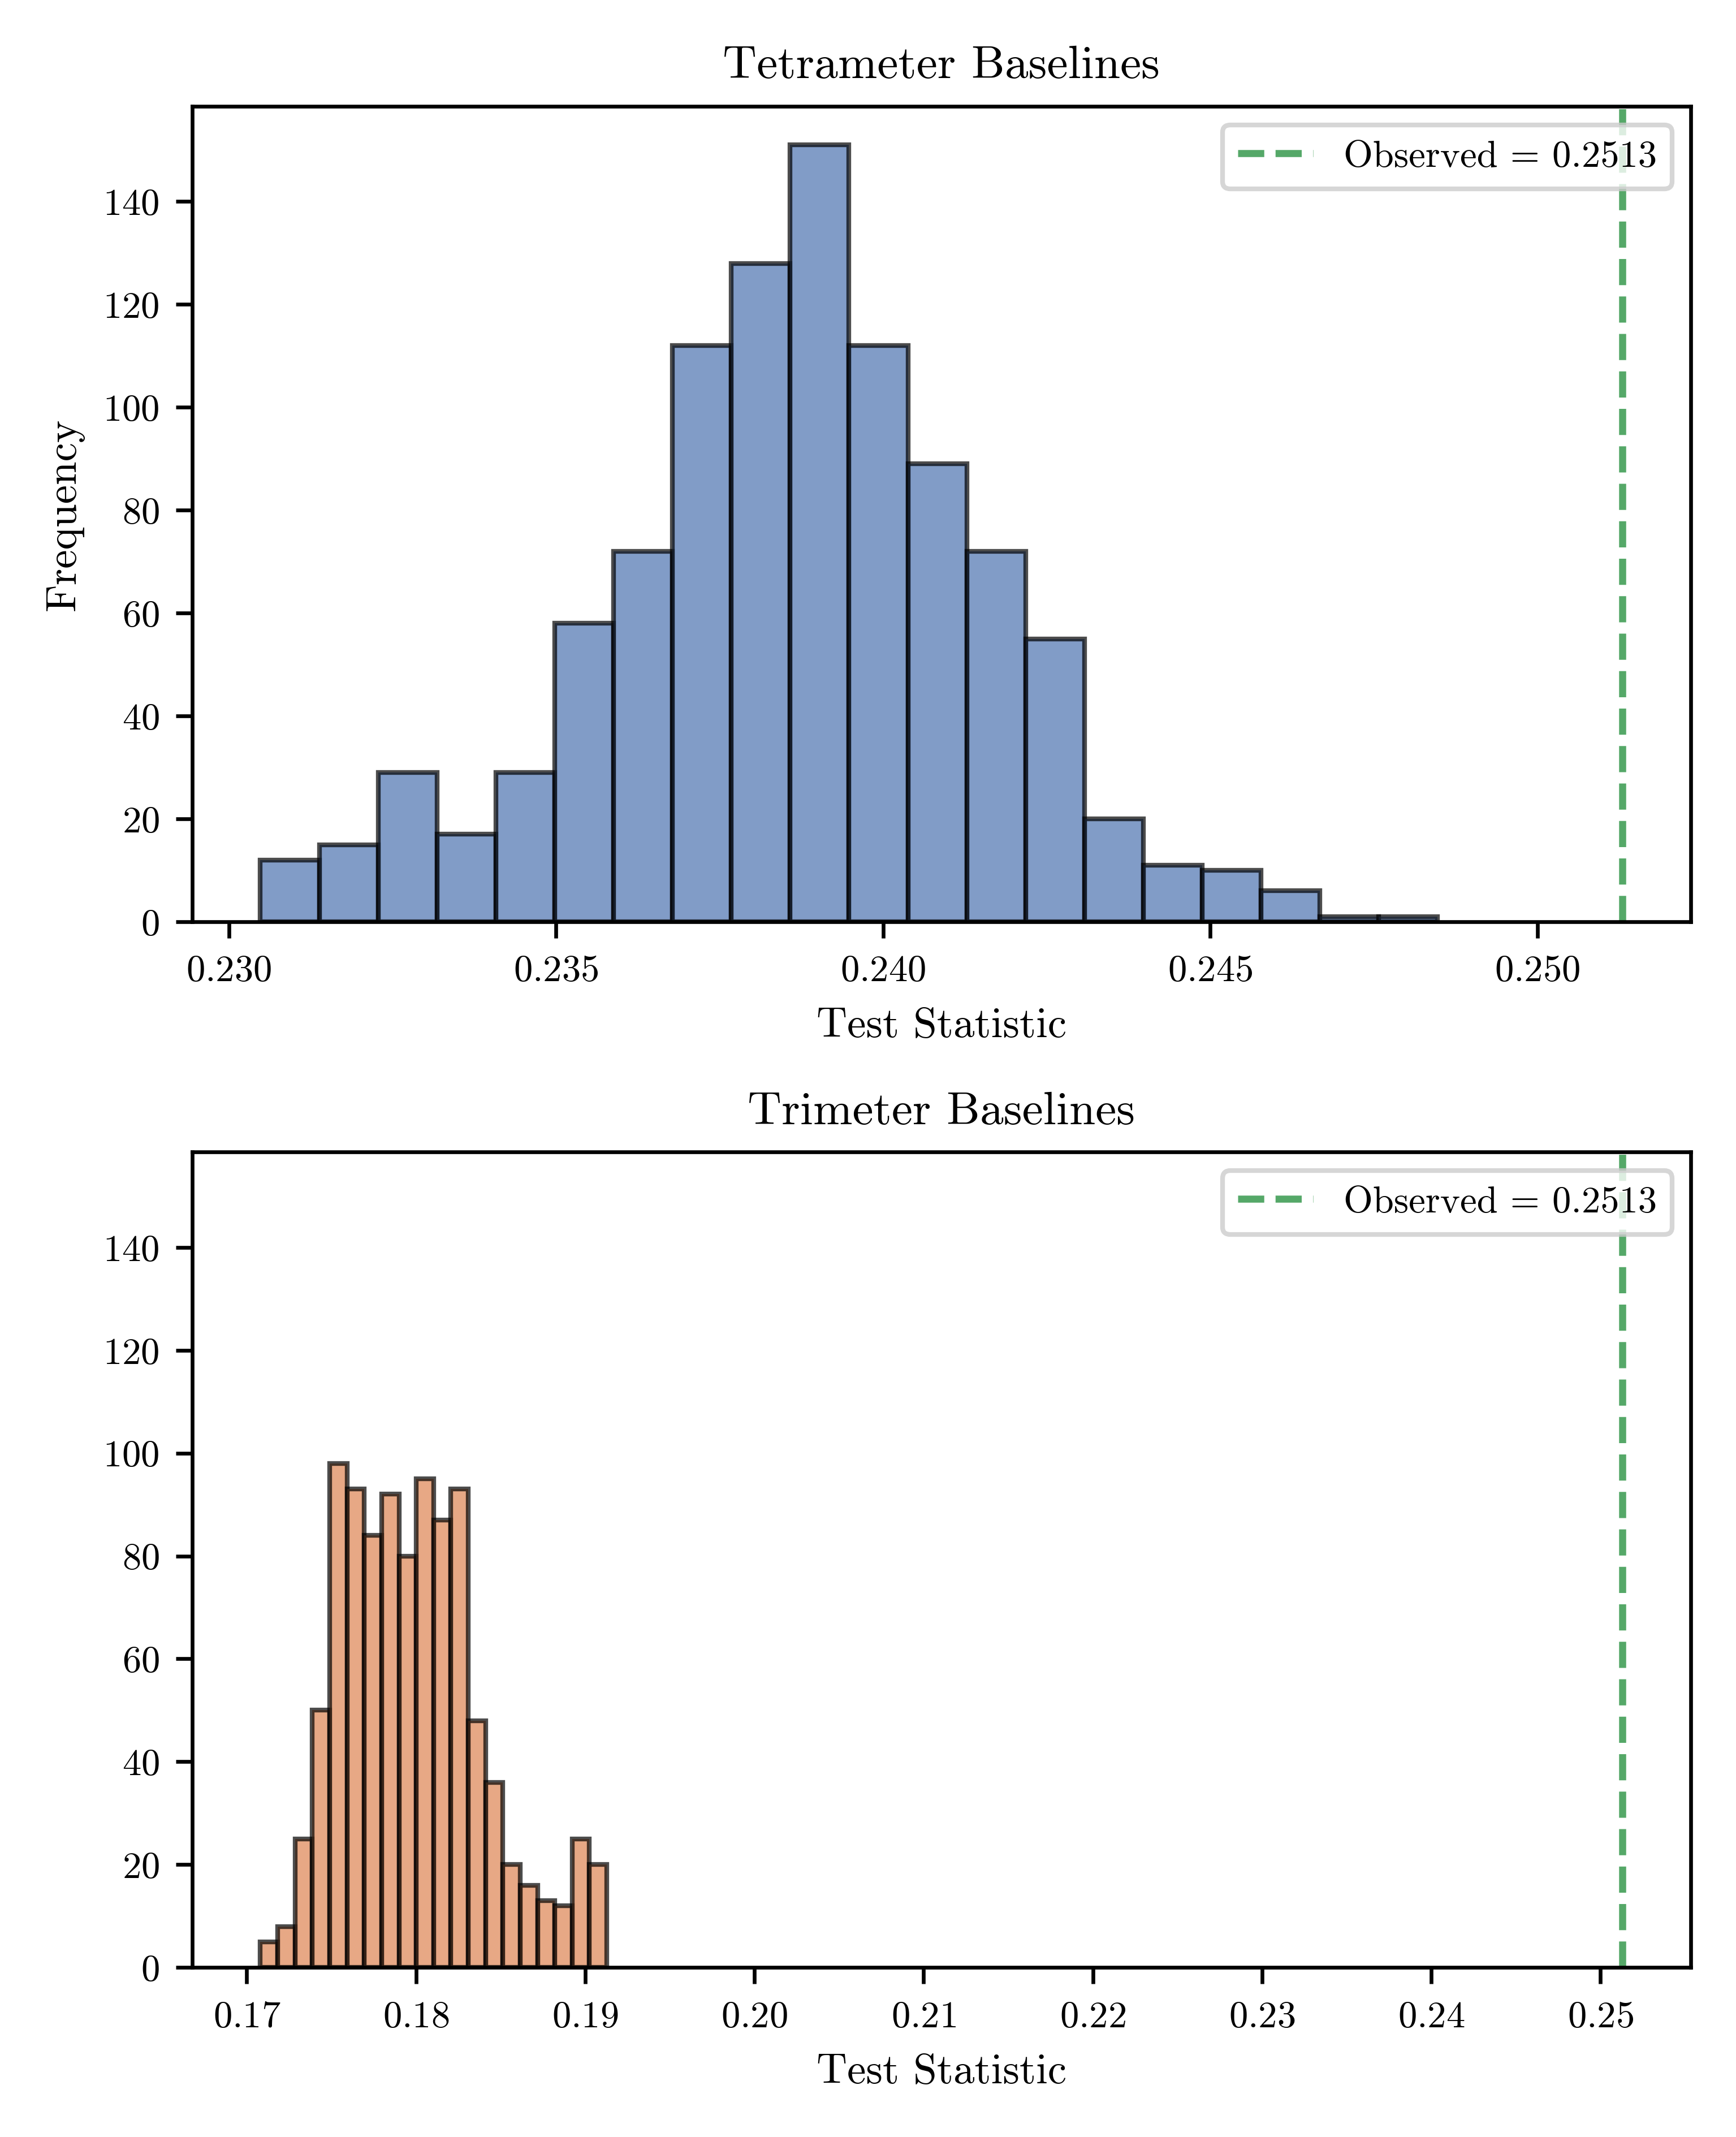
\includegraphics[width=1\linewidth]{figures/permutation_tests/orth_baseline_distributions.png}
    \caption{Distribution of expected values of the orthographic-accent metric}
    \label{fig:orth-perm}
\end{figure}

\begin{figure}
    \centering
    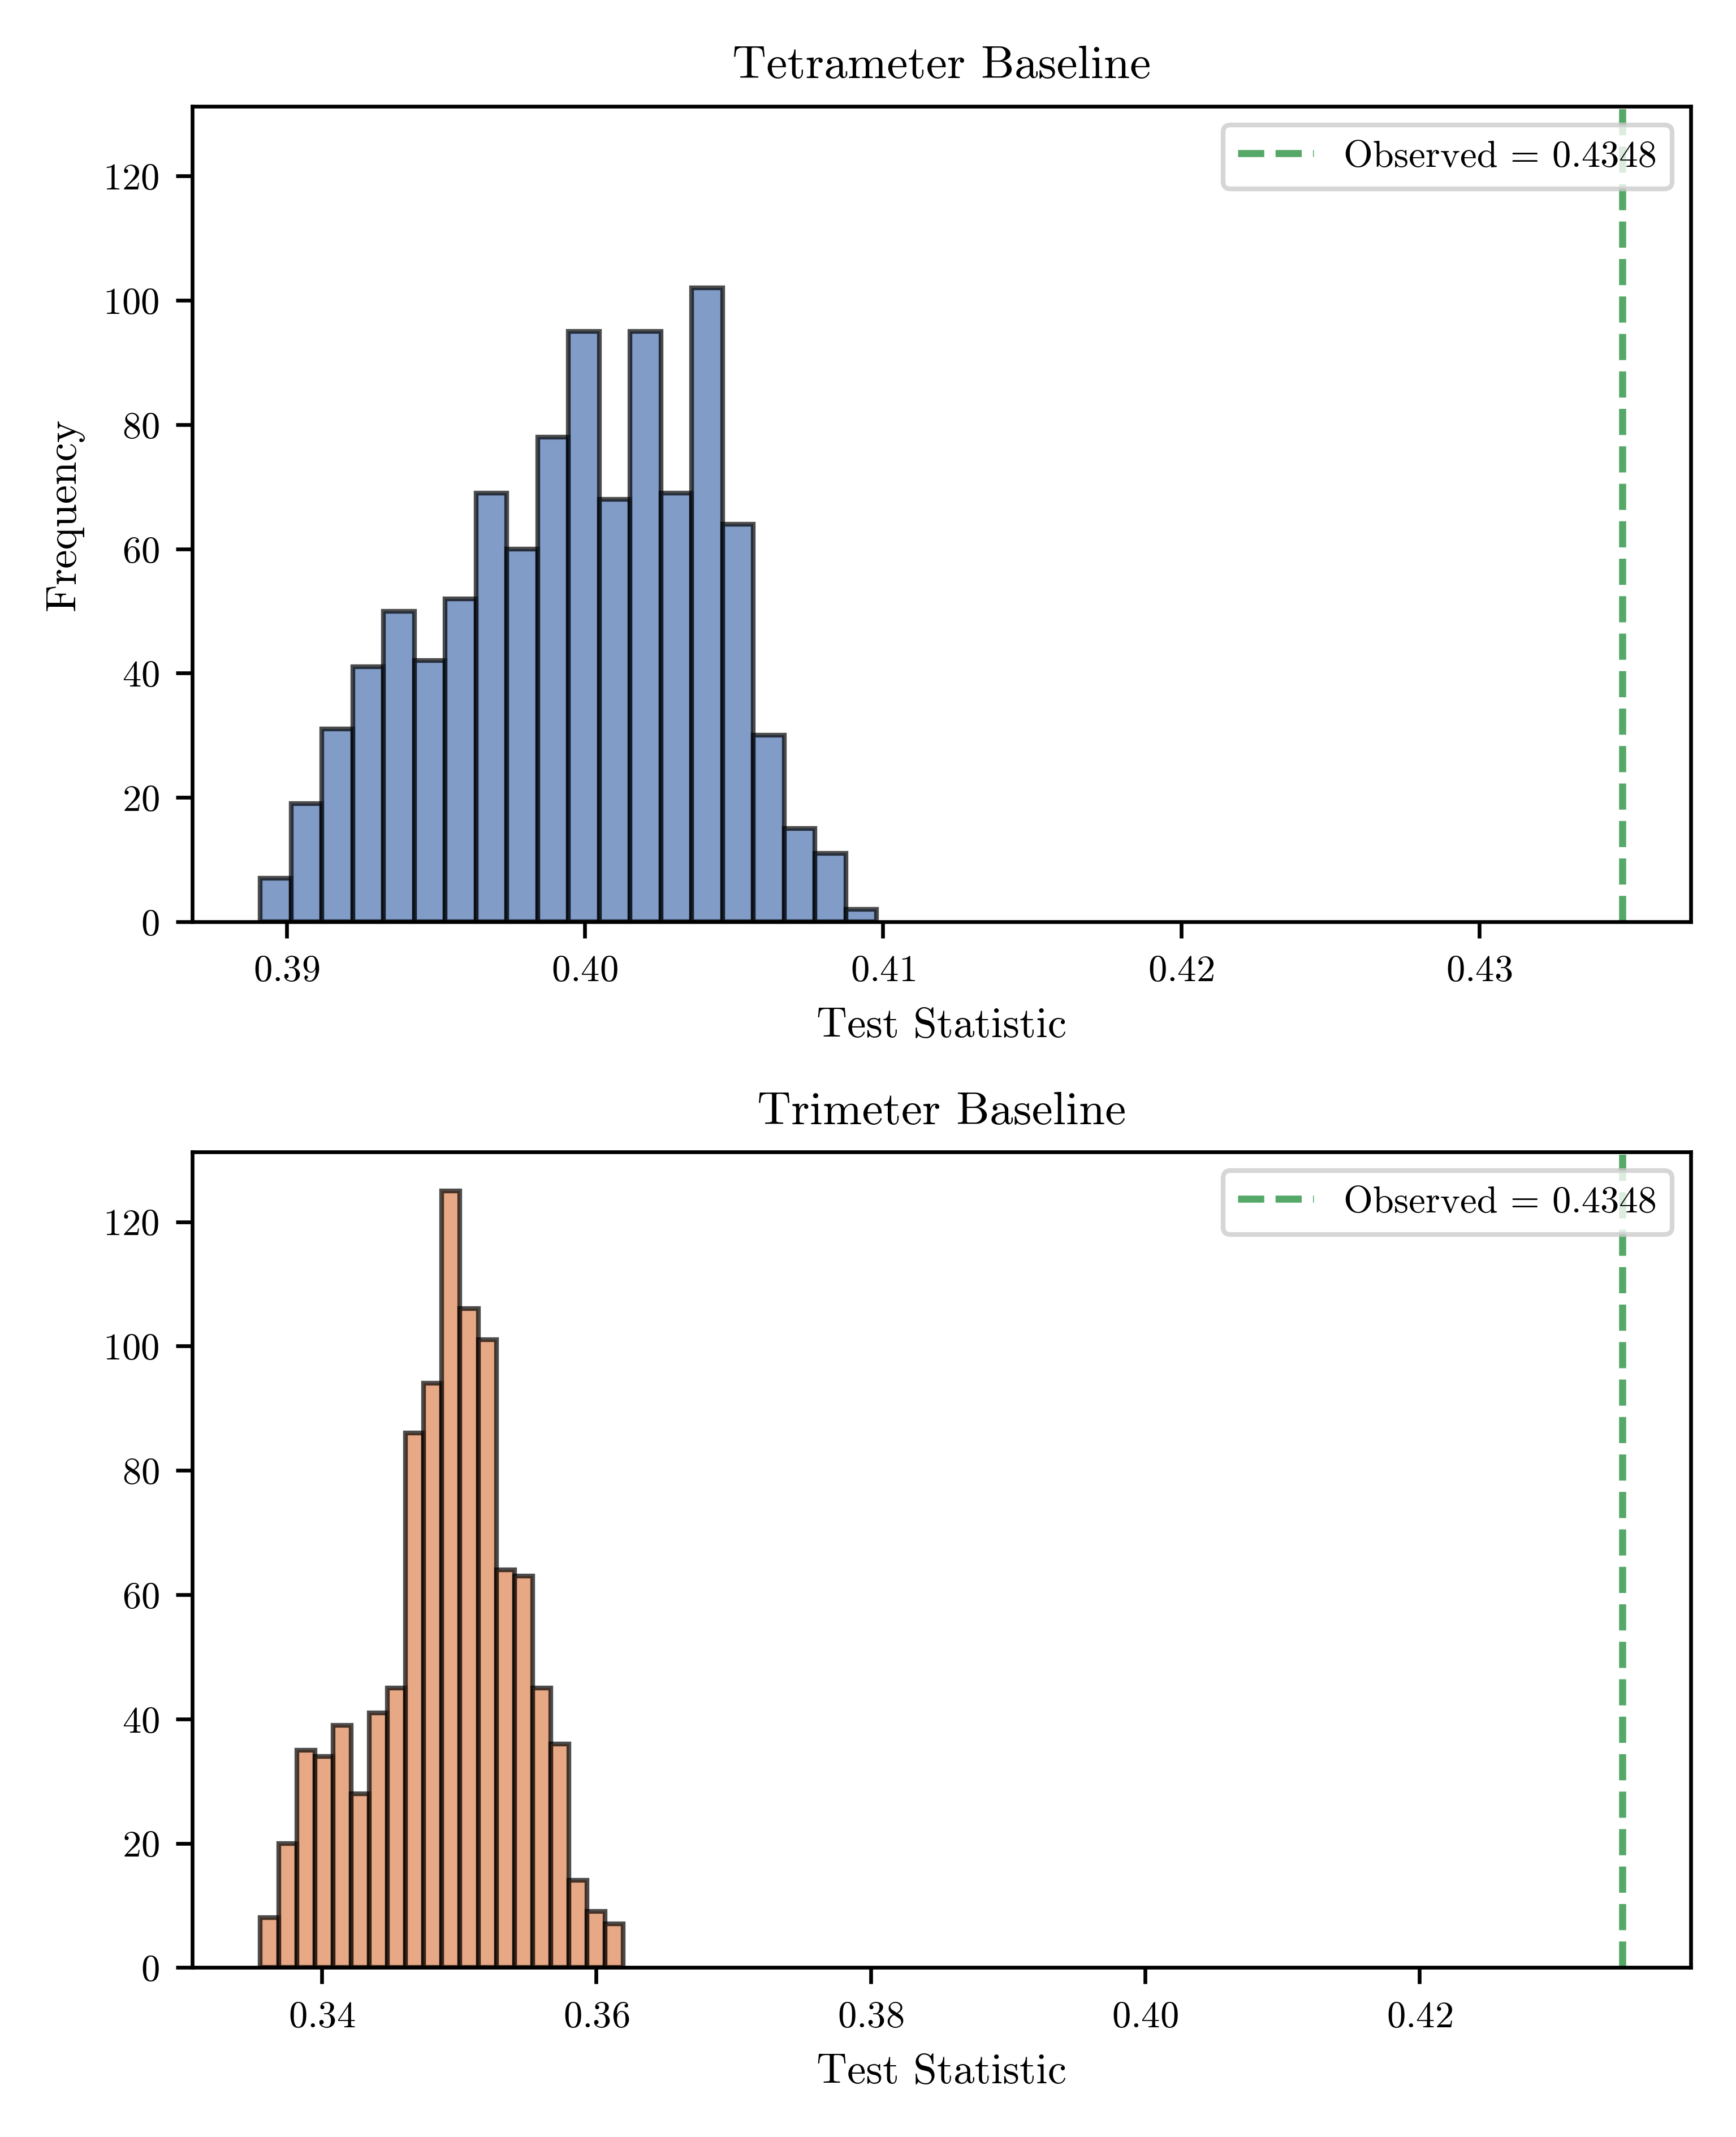
\includegraphics[width=1\linewidth]{figures/permutation_tests/barys_baseline_distributions.png}
    \caption{Distribution of expected values of the \textit{barys}-accent metric}
    \label{fig:barys-perm}
\end{figure}

\begin{figure}
    \centering
    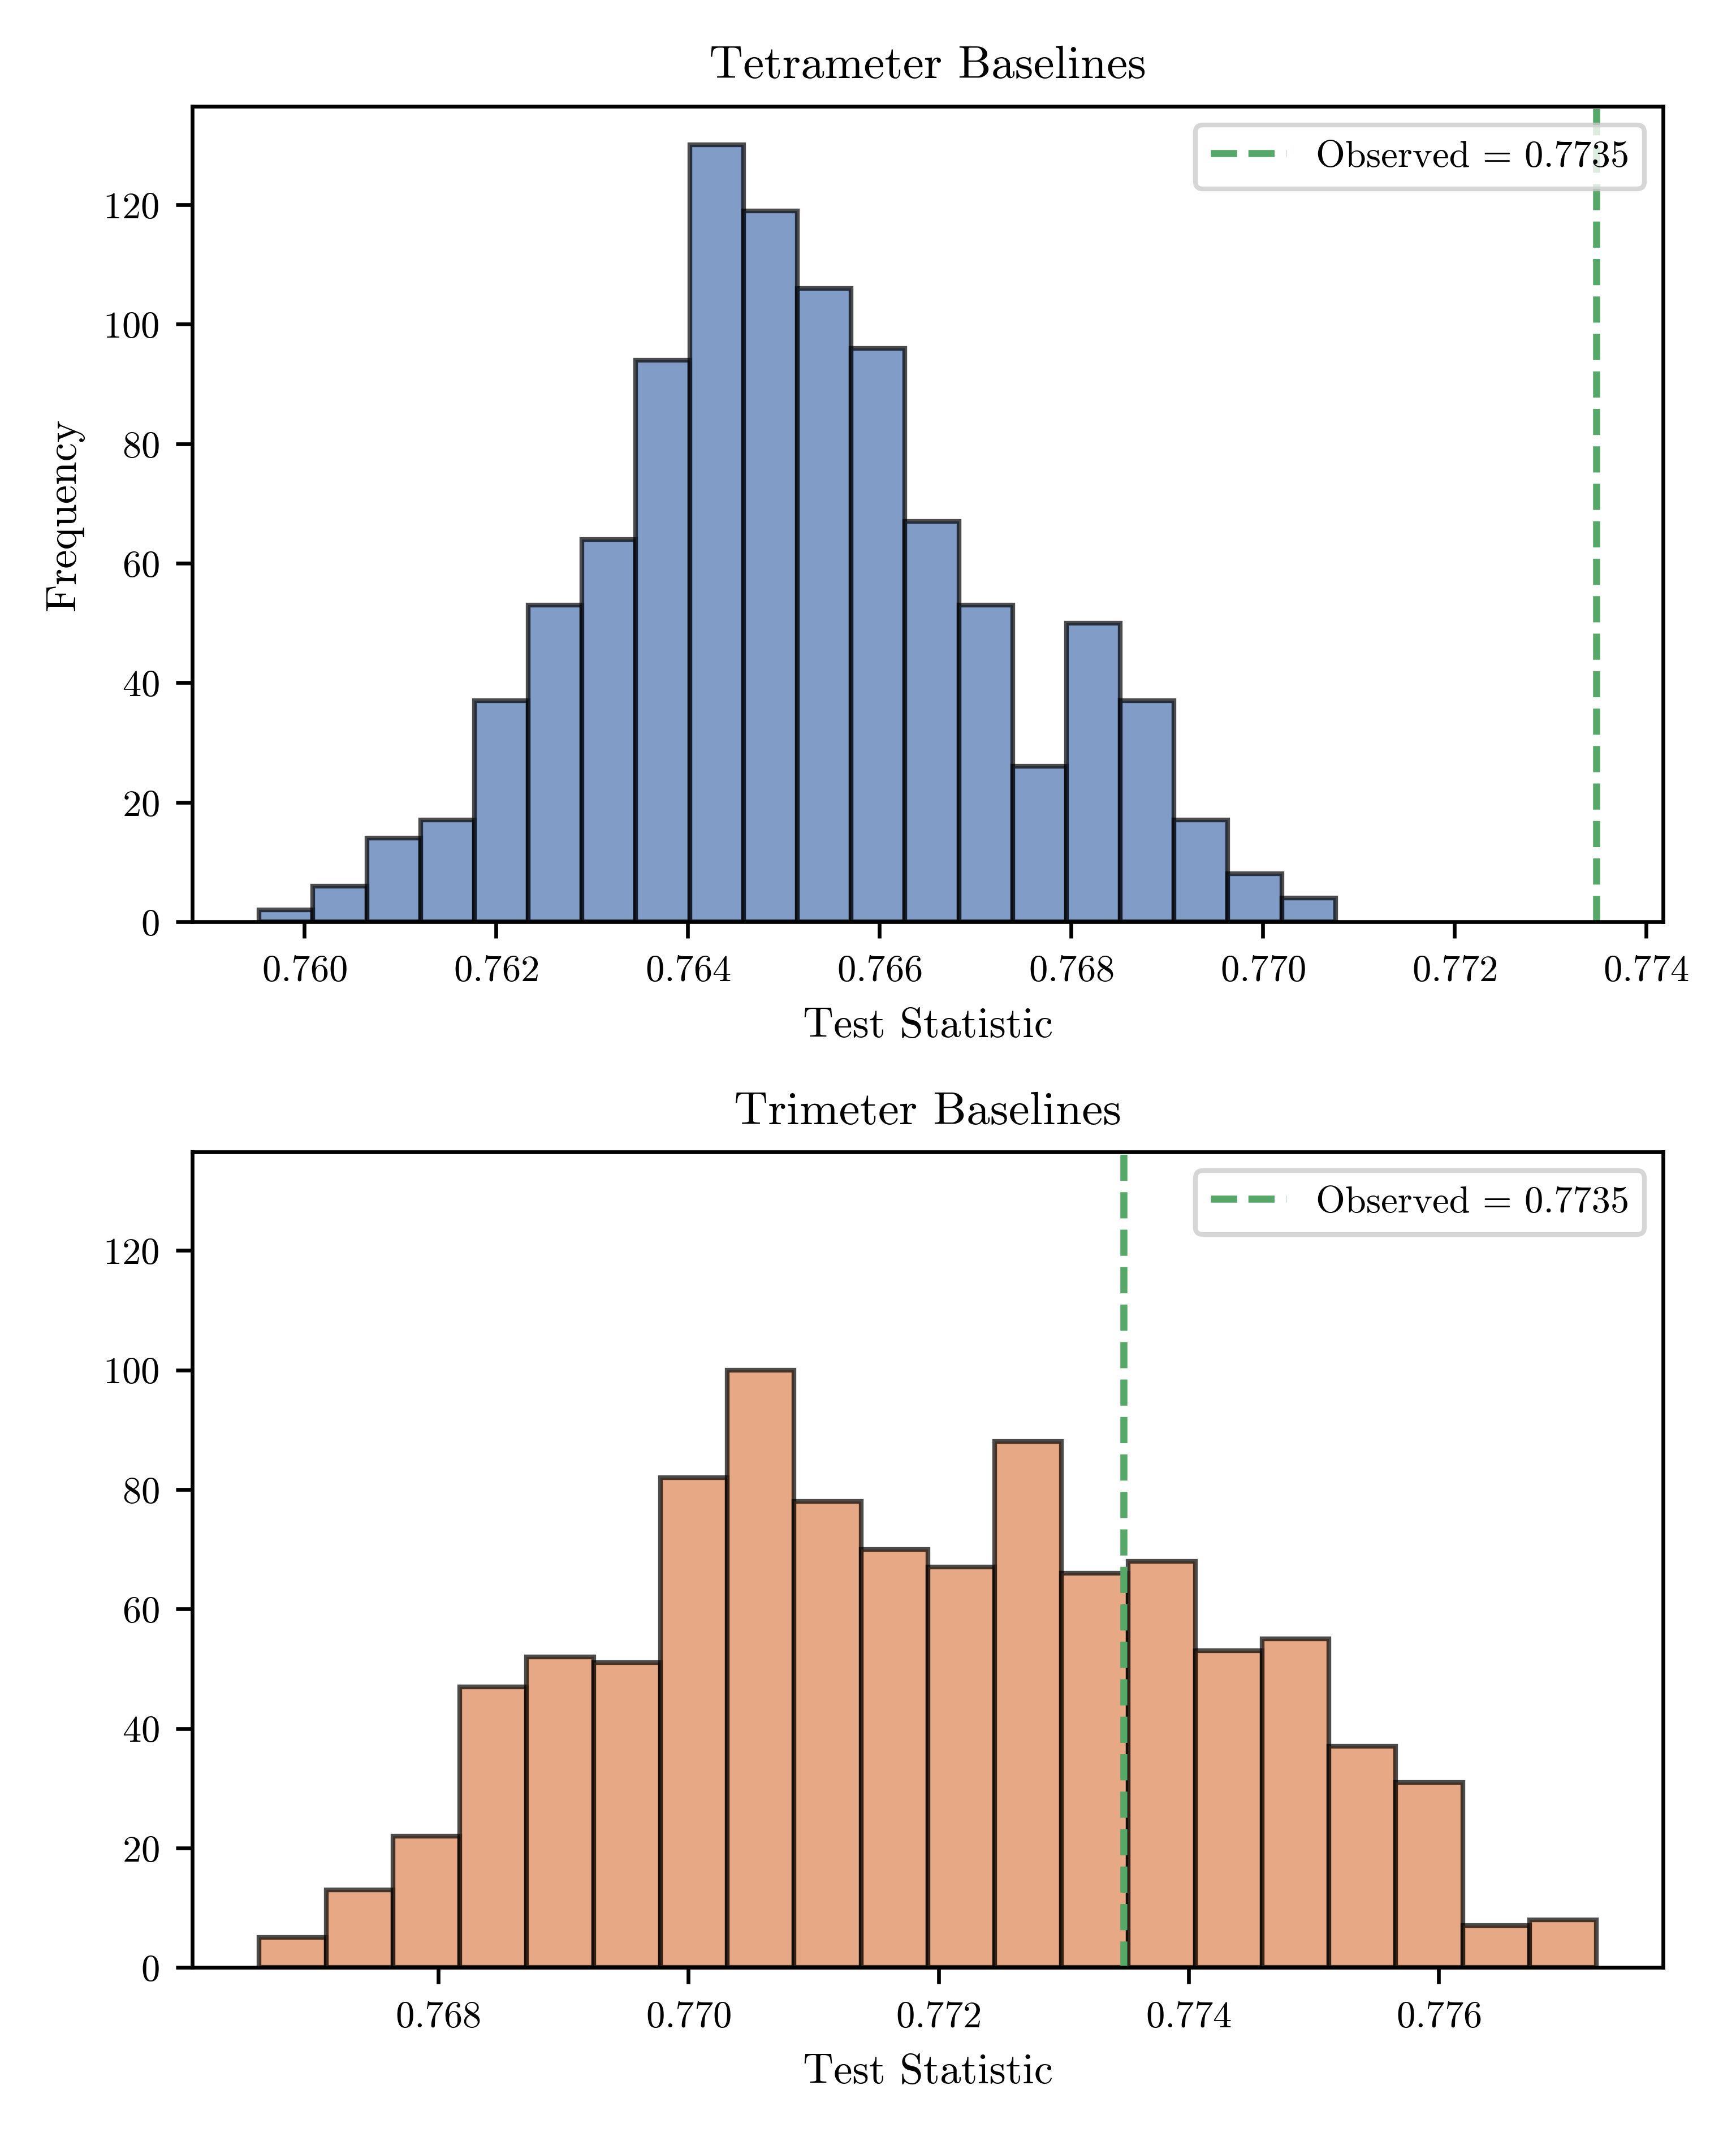
\includegraphics[width=1\linewidth]{figures/permutation_tests/comp_baseline_distributions.png}
    \caption{Distribution of expected values of the melodic-accent metric}
    \label{fig:comp-perm}
\end{figure}

In all tests but one, no expected values at all fall to the left of the observed value, which by definition means the lowest possible p-value in a one-sided permutation test of significance.\footnote{Such p-values are ``floored'' to $\frac{1}{1 + N}$, where $N$ is the number of permutations. Since those values are the same for all such tests, the only p-value that will need to be reported in \autoref{tab:perm} is the one that is not thus ``floored''.} But for the melodic metric against the trimeter baseline, the p-value is 0.26, which is firmly above 0.05, the standard threshold of significance. Aristophanes' refrains hence do not show more melodic compatibility than randomly paired comic iambic trimeters, while showing more than trochaic tetrameter.

This result is noteworthy and strange in two regards. First, because trochaic tetrameter is considered one of the most regular Greek metres, while comic trimeter one of the freest, a prediction corroborated by the results for the orthographic and \textit{barys} metrics, in both of which testing against the tetrameter is harder and yields a less significant result. Second, because it marks a decoupling of the third metric from the first two, suggesting that the metrics are indeed not measuring, as it were, the same underlying structure with concepts that are only superficially and nominally different. 

A way to quantify the results that are visible in the plots is to count how many standard deviations the observed value is from the mean of the expected values. These standard-deviation multiples, called z-values, are presented in \autoref{tab:perm}. 

\begin{table}[ht]
    \centering
    \begin{tabular}{l l l}
        \hline
                                             & Trimeter       & Tetrameter \\
        \hline
         $M_1$ (Acute-circumflex responsion) & $z = 17$       & $z = 4.3$ \\
         $M_2$ (\textit{Barys} responsion)   & $z = 16$       & $z = 8.1$ \\
         $M_3$ (Melodic compatibility)       & $z = 0.72$     & $z = 4.2$ \\
         \hline
    \end{tabular}
    \caption{Quantitative results of the permutation tests of significance}
    \label{tab:perm}
\end{table}

It is now possible to exactly describe the relationships between the significance of the metrics. $M_1$ and $M_2$ are both more than twenty-three times more standard deviations to the right of the expected mean of the trimeter baseline than $M_3$. Furthermore, the orthographic acute-circumflex responsion metric has a z-score one standard deviation better than the \textit{barys}, inverting the size of their raw observed values in \autoref{tab:general-results-no-pl}, serving as a reminder of the precariousness of interpreting data without tests. If counting responding acute and circumflex accents straight off the text surface yields a less noisy signal than preparing, calculating and counting the theoretical \textit{barys} accent metric—which of all three metrics is the most laborious, in that it requires text marked up with syllable weights–then the attractiveness of the \textit{barys} accent as a tool goes down.

\subsection{Line ends}

\begin{figure}
    \centering
    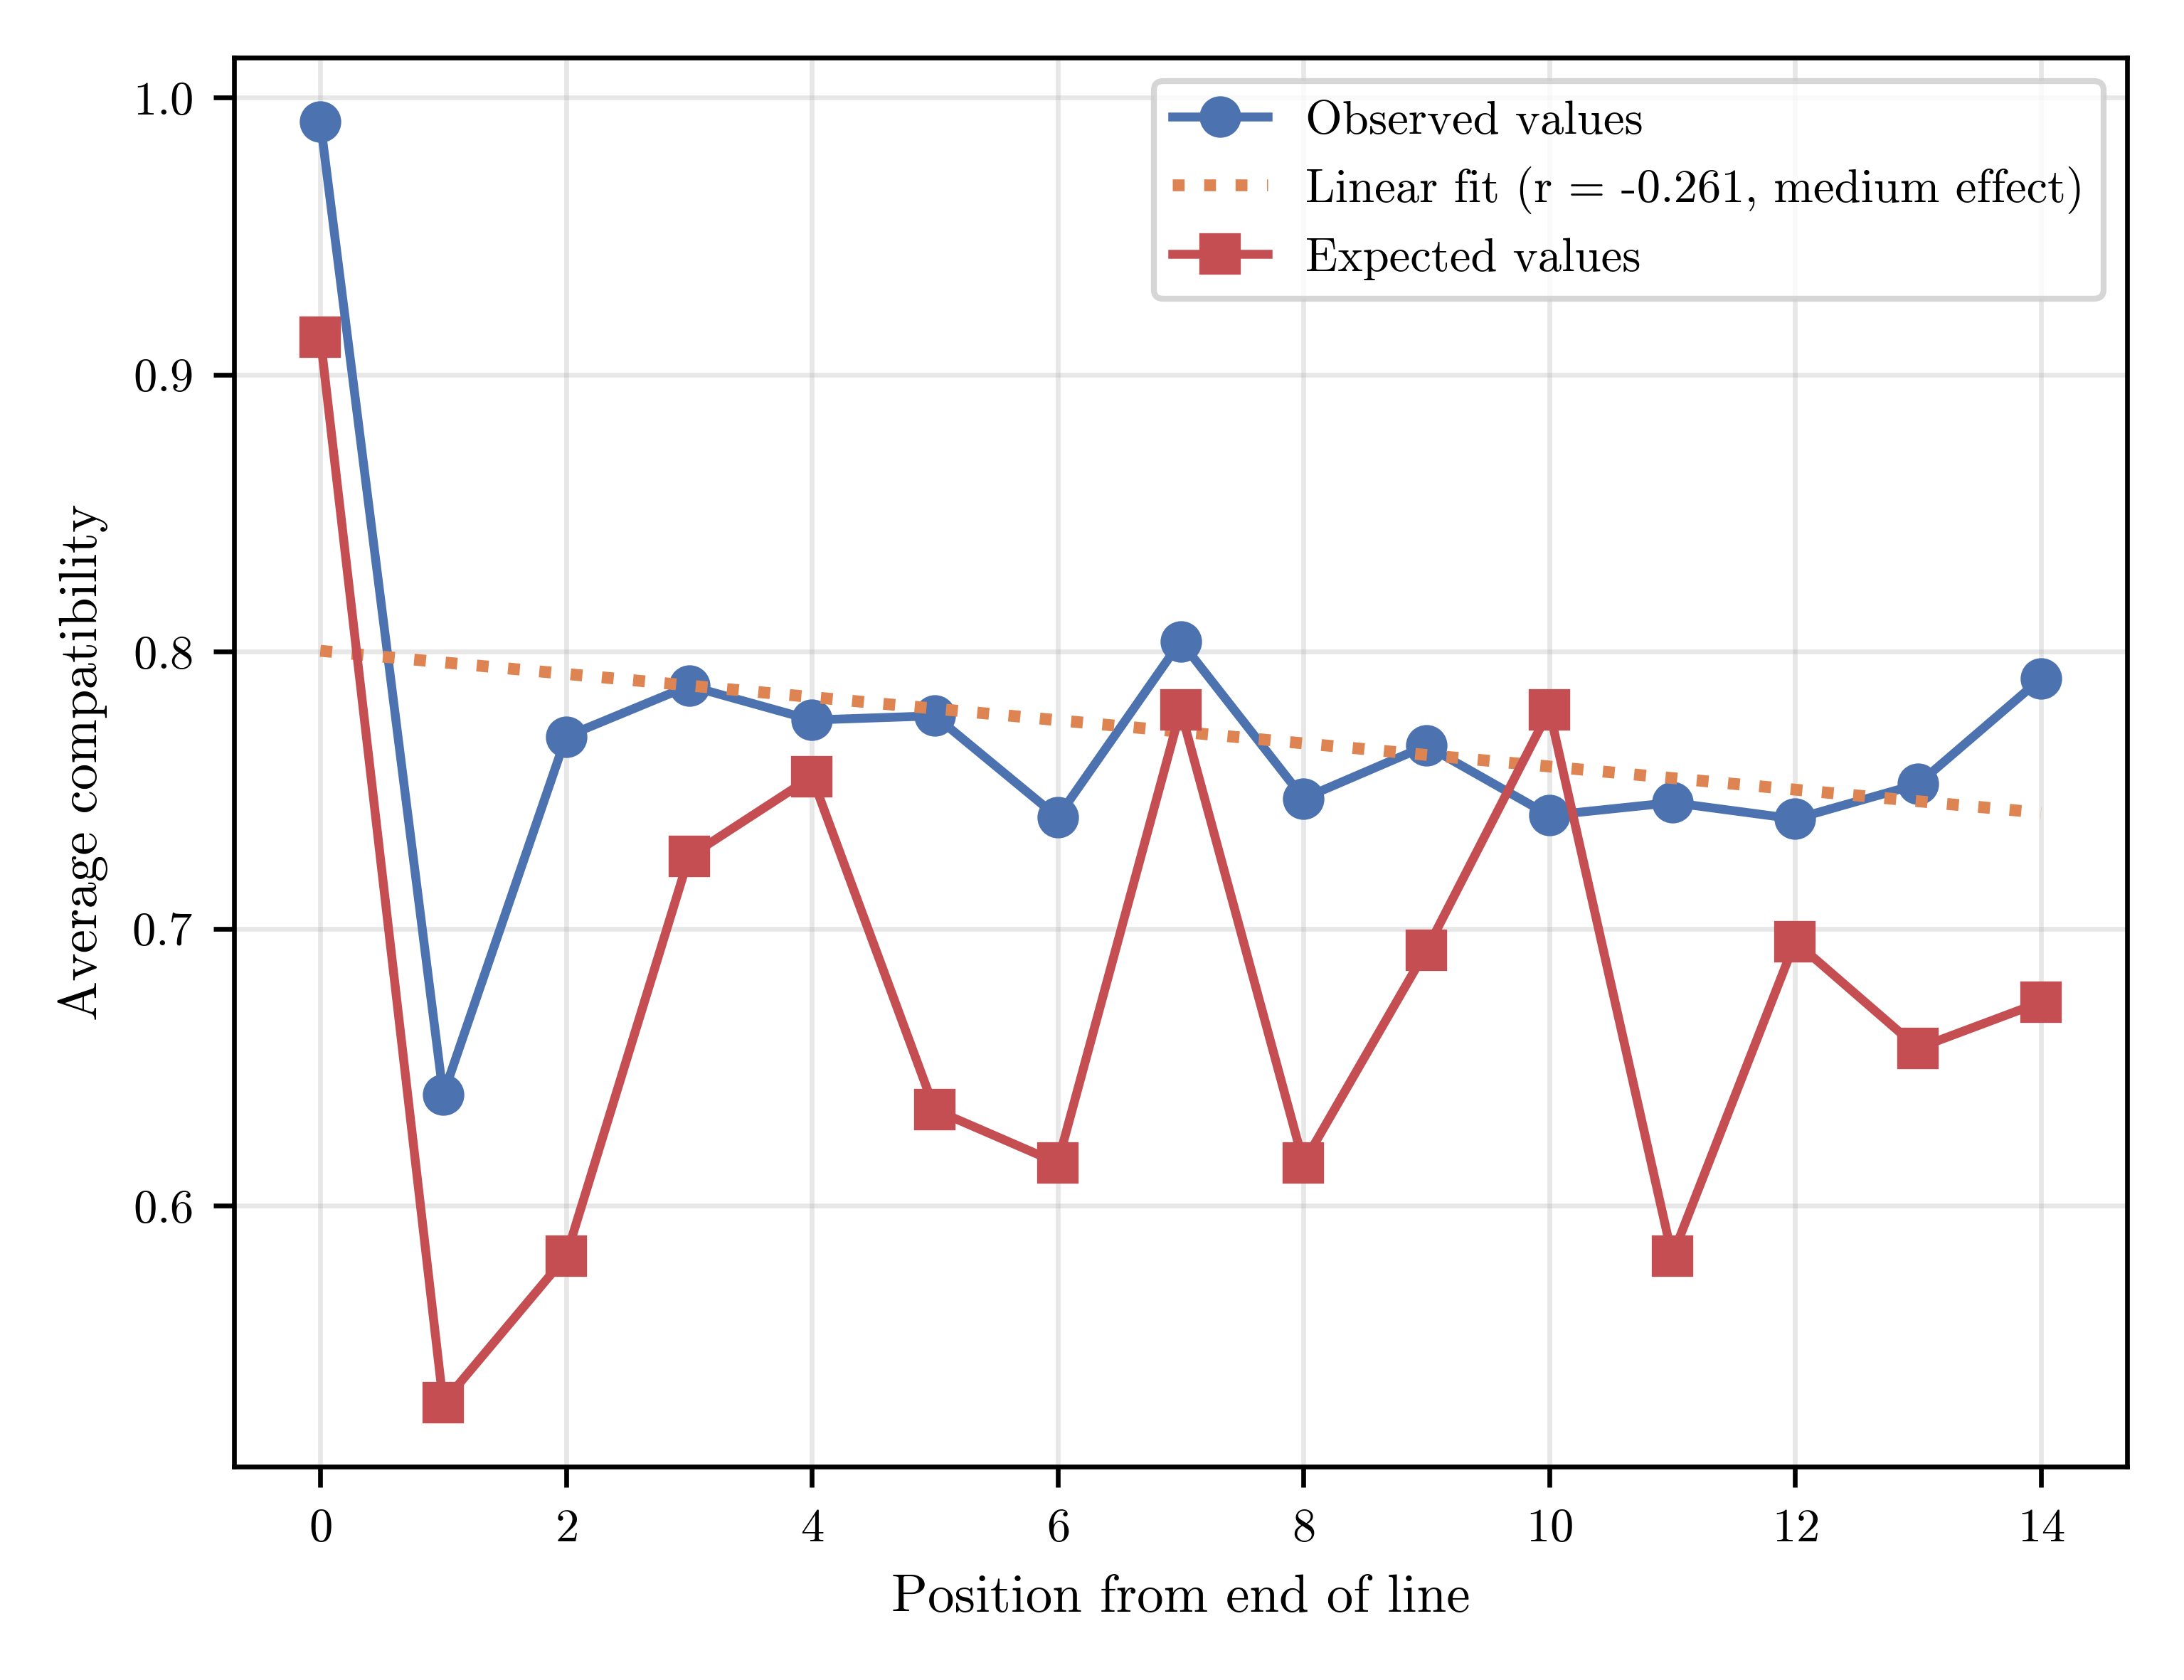
\includegraphics[width=1\linewidth]{figures/comp_line_end.png}
    \caption{Melodic compatibility by syllable, counting backwards from the end of the line}
    \label{fig:comp-line-end}
\end{figure}

By plotting melodic compatibility in \autoref{fig:comp-line-end} as a function of syllable index counting backwards from the end of the line for both Aristophanes corpus and the baselines it is easy to falsify any attribution of significance to the hypothesis that the line end is a locus of intentional accentual responsion. The spike in compatibility is an effect of the natural constraints of the language and/or versification.

\section{Melodic Compatibility and Genre: Interpretation of the Comparative Results for Metric 3}

The overall scores in \autoref{tab:general-results-no-pl} made it look like Aristophanes' melodic compatibility was only slightly less than Aeschylus' and Sophocles'. That is emphatically not the case, which is made intuitively clear in \autoref{fig:histogram-three}, where the $M_3$ play scores of each poet are separately ordered by size so that the difference in score between the most melodically compatible plays of each poet are immediately graspable. In the top four ranks, Sophocles' plays are consistently closer to Aeschylus' respectively ranked plays than they are to Aristophanes'. 

\begin{figure}
    \centering
    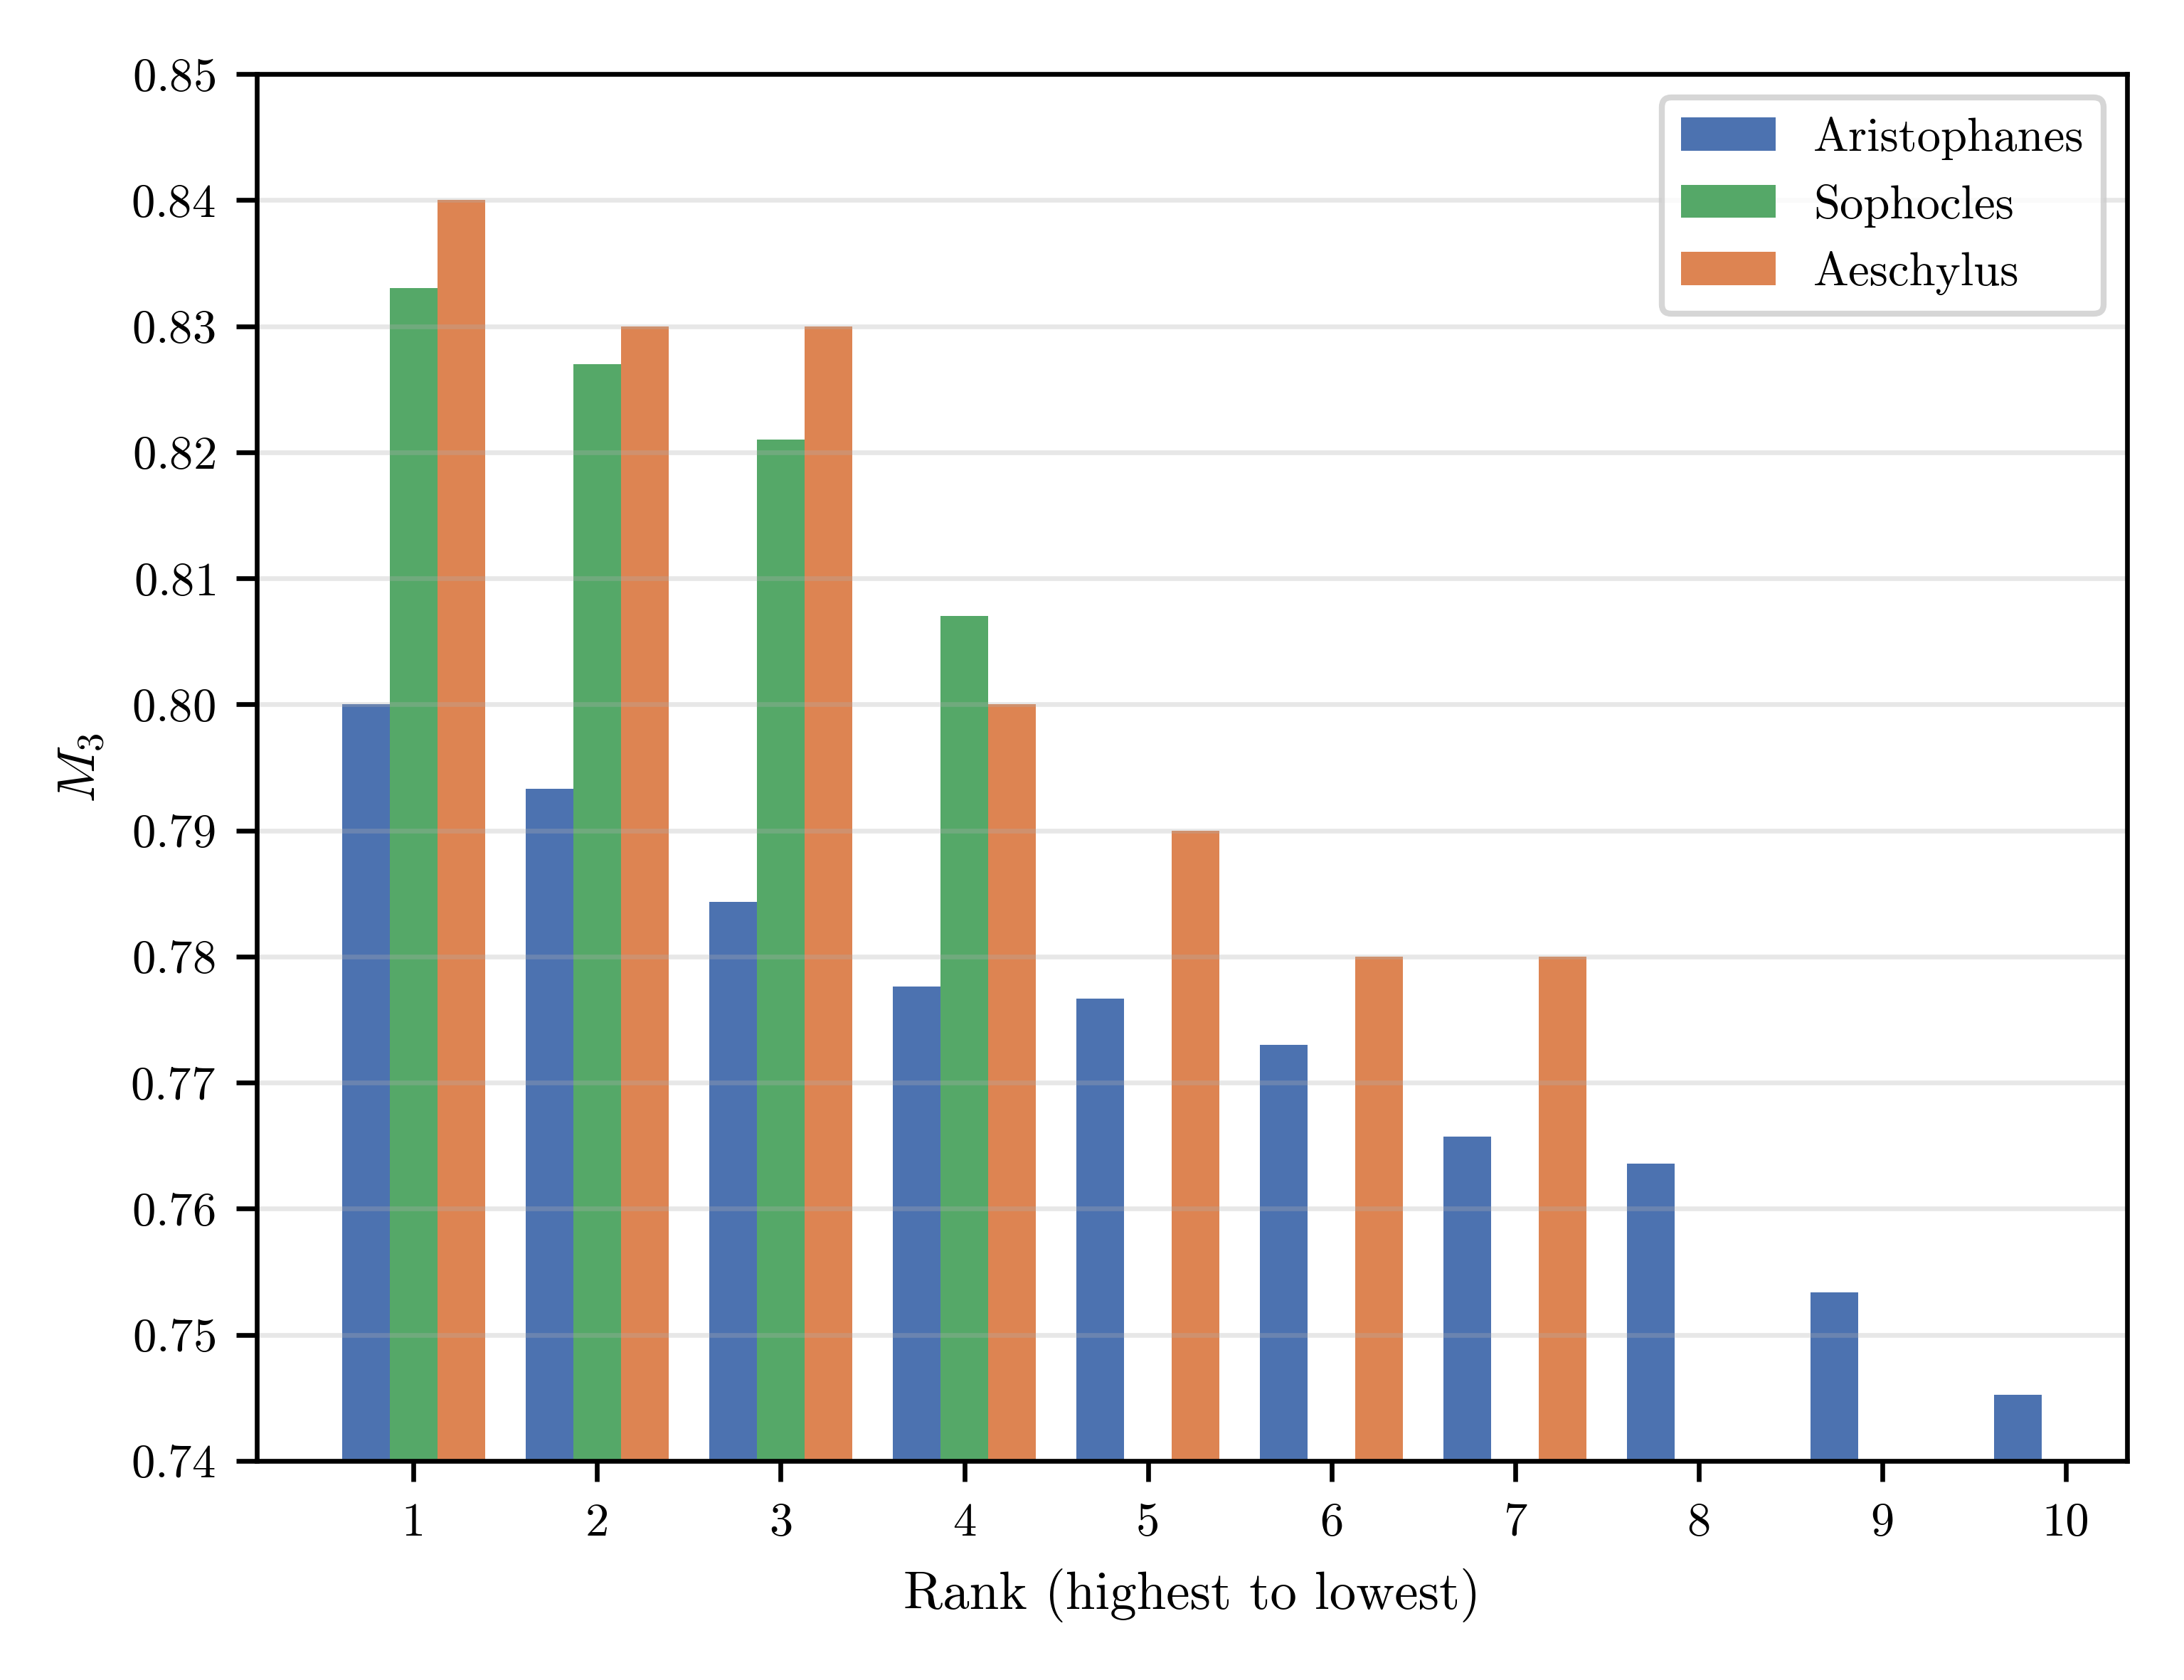
\includegraphics[width=1\linewidth]{figures/histogram_three.png}
    \caption{Comparison between orderings of the $M_3$ play scores of Ar., Soph.\ and Aesch.}
    \label{fig:histogram-three}
\end{figure}

In an article that constitutes the state of the art of statistical evidence for the development of accentual responsion during the fifth century, Conser writes:
\begin{quote}
    The tendency toward increasing accentual responsion in both Aeschylus and early Sophocles suggests that melodies became more lively during the fifth century BCE, anticipating the rise of the “New Music” at the century’s end. \parencite[110-111]{conserAiolaNuxMusical2024}
\end{quote}

My new results complicate this situation, by presenting evidence of a decline in accentual responsion during the last three decades of the fifth century B.C.\ and the first decade of the fourth.\footnote{Ignoring \textit{Plutus}, Aristophanes' corpus spans from the premiere of the \textit{Acharnienses} in 425 B.C.\ to the \textit{Ecclesiazusae} in 391 B.C.}

There are two possible but mutually exclusive ways to react to this finding. The first reaction is to hypothesize that the development of accentual responsion (and perhaps ``liveliness'', in Conser's interpretation) in lyric peaked at around the time of Aeschylus' later career and the career of his younger rival Sophocles, only for the pendulum to swing back during the career of Aristophanes: it is striking how Aristophanes' scores are all in the span of $0.78\pm2$, centred around the score of Aeschylus' first play. This hypothesis rhymes ill with the general account of ``New Music'' and its association with Aristophanes' contemporaries Euripides and Timotheus of Miletus.

The second possible reaction is to instead take the divergence as marking the presence of a real stylistic genre boundary. Confining the positive trend to tragedy, the hypothesis would here be that Old Comedy was markedly melodico-prosodically conservative, in a way that perhaps harkened back to an earlier style of drama, preserved for us in the first plays of Aeschylus.

\textit{Prima facie}, the second hypothesis appears the more attractive one, not because of scholarly momentum, but primarily because the contents of Aristophanes' plays generally betray a reactionary stance in art, culture and politics, and in particular are peppered with both numerous jabs at the musical innovations of Euripides and his ``New Music'' peers, and numerous praises of Aeschylus and other artists of the previous generation.\footnote{For a summary of Aristophanes' and others' \textit{testimonia} on the ``New Music'', see \textcite{dangourNewMusicWhats2006} and \textcite{dangourOldNewMusic2020}. \textcite{comottiMelodiaAccentoDi1989} does a small Wahlström-style analysis of accentual responsion in Aeschylus, Sophocles and Euripides and sees a general diachronic decline.} The genre hypothesis also chimes well with modern ethnomusicology, where a recent review of three different studies in \textcite[271]{schellenbergDoesLanguageDetermine2012}, mentioned in \autoref{sec:comparative}, showed that genre and performance context can be predictors of whether music respects accents, and that adherence to tradition is not necessarily a positive such predictor.

Final adjudication between these two options can only be done in the light of more data, and will have to be postponed until further research is done.

%===============================================================
% Conclusion

\section{Conclusion}

Let me end by reiterating the most noteworthy results and indicate natural vectors of continued research. 

To begin with, I have showed that the ``sacred precinct'' of the Graces is in better condition than previously known, since a significant echo of Aristophanes' melodic scaffolding has survived. Furthermore, Wahlström's hypothesis has been fully dragged out of the closet and vindicated, as five out of six significance tests passed, although his specific hypothesis regarding line ends has been exposed as but the noise of linguistic constraints.

The picture of the relationship between responsion based on ``naive'' accent counting and that based on \textit{barys} accent counting has been complicated, as it has been shown that the former is strictly better for proving the significance of Aristophanes' use of accentual responsion. Getting a higher observed score is not a merit for a metric if the baseline scales equally fast or even faster.

Last but not least, and perhaps most importantly, new light has been shone on the relationship between Aristophanes and the tragedians that holds potential to either upend certain widely held beliefs regarding fifth-century lyric and its major diachronic trends, if one chooses to interpret the decline in Aristophanes as breaking the trend, or usher in a new prosodical approach to genre, if one takes it as a trait of comedy. Either way, the philological and statistical tools used in this article open new avenues for data-driven research into hitherto cryptic dimensions of Greek lyric, using the accentual veneer to uncover information that has escaped those looking too deeply:

\begin{quote}
Oh, those Greeks! They knew how to live: what is needed for that is to stop bravely at the surface, the fold, the skin; to worship appearance, to believe in shapes, tones, words - in the whole Olympus of appearance! Those Greeks were superficial - \textit{out of profundity!} \parencite[8]{nietzscheGaySciencePrelude2004}
\end{quote}

\section*{Data Availability Statement}
All the code, data and results used in this paper are available open-source at the accompanying Zenodo repository \textcite{albinthornclelandUrdatornAristophaniscanticaArticle2026}. The core functions calculating melodic contour contain adapted snippets of code from Anna Conser’s open-source Github project ``Greek-Poetry''.\footnote{\url{https://github.com/aconser/Greek-Poetry}}

\section*{Acknowledgments}
Thank you to the participants of the presentation of an early version of this research at the higher seminar in Uppsala in early 2025, and to the participants and organizers of Plotting Poetry 8 for an inspiring stay in Prague.

%===============================================================
% Bibliography
\printbibliography

\end{document}
